\documentclass[11pt, french]{report-rd-info}
   % - 12pt:  peut être préférable pour faciliter la lecture sur les petits écrans, demander à l'encadrement
   % - screen:  à enlever pour obtenir un rapport au format A4
   % - french:  à remplacer par english en cas de rédaction (exceptionnelle) en anglais
\usepackage[utf8]{inputenc}
   % - latin9, utf8, etc.
\usepackage[T1]{fontenc}

% définitions propres au contenu actuel
\usepackage{enumerate}
\usepackage{amsmath, amssymb}
\usepackage{algorithm}
	\floatname{algorithm}{Algorithme}
	\ifenglish
      \renewcommand{\listalgorithmname}{List of Algorithms}
	\else
	   \renewcommand{\listalgorithmname}{Liste des algorithmes}
	\fi
\usepackage{algorithmic}
	\renewcommand{\algorithmicrequire}{\textbf{Précondition:}}
	\renewcommand{\algorithmicensure}{\textbf{Post-condition:}}
	\renewcommand{\algorithmiccomment}[1]{\emph{// #1}}
	\renewcommand{\algorithmicend}{\textbf{fin}}
	\renewcommand{\algorithmicif}{\textbf{si}}
	\renewcommand{\algorithmicthen}{\textbf{alors}}
	\renewcommand{\algorithmicelse}{\textbf{sinon}}
	\renewcommand{\algorithmicelsif}{\algorithmicelse\ \algorithmicif}
	\renewcommand{\algorithmicendif}{\algorithmicend\ \algorithmicif}
	\renewcommand{\algorithmicfor}{\textbf{pour}}
	\renewcommand{\algorithmicforall}{\textbf{pour chaque}}
	\renewcommand{\algorithmicdo}{\textbf{faire}}
	\renewcommand{\algorithmicendfor}{\algorithmicend\ \algorithmicfor}
	\renewcommand{\algorithmicwhile}{\textbf{tant que}}
	\renewcommand{\algorithmicendwhile}{\algorithmicend\ \algorithmicwhile}
	\renewcommand{\algorithmicloop}{\textbf{fin tant que}}
	\renewcommand{\algorithmicendloop}{\algorithmicend\ \algorithmicloop}
	\renewcommand{\algorithmicrepeat}{\textbf{répéter}}
	\renewcommand{\algorithmicuntil}{\textbf{jusqu'à}}
	\renewcommand{\algorithmicprint}{\textbf{afficher}}
	\renewcommand{\algorithmicreturn}{\textbf{renvoyer}}
	\renewcommand{\algorithmictrue}{\textbf{vrai}}
	\renewcommand{\algorithmicfalse}{\textbf{fraux}}

\newenvironment{typographie}{\begin{quote}\textbf{Typographie}. }{\end{quote}}
\newenvironment{structuration}{\begin{quote}\textbf{Structuration}. }{\end{quote}}

\newtheorem{theoreme}{Théorème}
\newtheorem{preuve}{Preuve}

\begin{document}

\title{Magic Portrait}
\subtitle{Améliorons la photographie (de portrait) !}
\authorA{Pierre-Yves}{Hervo}
\authorB{Paul-François}{Jeau}
\supervisor{Matthieu}{Perreira Da Silva}
   % Si plusieurs co-encadrants, alors utiliser la forme suivante :
   %    \cosupervisor{Alter}{Ego \& {\normalfont Jean} Cadre}
\coordinator{Nom}{Prenom}
\institution{IRCCyN}
   % - LINA pour un encadrement par les membres des équipes GRIM et COD (voire d'autres) ;
   % - IRCCyN pour un encadrement par les membres des équipes IVC ;
   % - XXX pour un encadrement dans le cadre d'un autre organisme
   %   (il faut alors fournir dans le répertoire "logos" les fichiers correspondant : XXX.pdf -- à défaut XXX.jpeg ou XXX.png -- pour pdflatex *et* XXX.eps pour latex) ;
   % - commenter pour un encadrement qui relève d'un travail de recherche non affecté à une équipe.
\theme{IVC}
   % - à fournir dans le cas d'un laboratoire (GRIM, COD ou IVC pour les équipes du département)
   % - commenter autrement
   % - ne peut pas être fourni si l'institution n'a pas été renseignée
%\coinstitution{Centre national de la recherche scientifique}{CNRS}{1.7cm}
   % - pour ajouter un partenaire
   % - le logo doit correspondre au fichier déclaré, ici CNRS.pdf.
   % - le troisième paramètre permet d'adapter la largeur du logo afin
   %   de le rendre visuellement comparable à ceux mis par défaut (université de Nantes et
   %   éventuellement laboratoire)
\date{18 novembre 2013}
   % - en français les mois ne prennent pas de majuscule (sauf si vous ne mettez pas le jour)
   % - inutile de mettre un 0 devant les jours 1 à 9 du mois !
   % - le jour est peut-être même une précision inutile...

%-------------------------------------------------------------------------------------------------------------

\begin{abstract}
%\small % À décommenter si le résumé est légèrement trop long pour tenir dans la page
Comme son nom l'indique, le résumé condense en quelques paragraphes
la \emph{totalité} du rapport. Il faut donc décrire succinctement et
successivement :
\begin{enumerate}
   \item le sujet et la problématique ;
   \item les objectifs fixés ;
   \item les recherches effectuées ;
   \item les décisions prises ;
   \item les constructions conceptuelles ;
   \item les développements accomplis ;
   \item les expérimentations conduites, leurs résultats et leur interprétation ;
   \item les limites de ce travail ;
   \item les perspectives qu'il ouvre.
\end{enumerate}
\end{abstract}

\begin{classification}
%\small % Idem
   Des éléments d'indexation bibliographiques \emph{doivent} être fournis. Ci-dessous est illustrée l'usage du thésaurus de l'ACM avec les catégories codifiées et des éléments d'indexation ouverts.
   Suivre le modèle de l'ACM : cf. \url{http://www.acm.org/class/1998/}

   \category{H.2.8}{Database Applications}{Image databases}
   \category{H.3.3}{Information Search and Retrieval}{Clustering, Information filtering, Relevance feedback}
   \category{H.3.7}{Digital Libraries}{User issues}
   \category{I.5.3}{Clustering}{Algorithms, Similarity measures}
   \category{I.4.10}{Image Representation}{Statistical, Multidimensional}
   \terms{Des mots clés couramment employés et très généraux sont à ajouter aux catégories. ex.\ : Algorithms, performance, experimentation, human factors, verification.}
   \keywords{Des mots clés supplémentaires et très spécifiques peuvent être ajoutés. ex.\ : Personnalisation, recherche d'images par le contenu, classification, rétro-action,
   apprentissage.}
\end{classification}

\maketitle

%-------------------------------------------------------------------------------------------------------------

\begin{acknowledgements}
Nous souhaitons remercier Mathieu PERREIRA DA SILVA pour son encadrement et ses conseils tout au long de cette première phase du projet de Recherche et Développement.
De plus, nos remerciements s'adressent aussi à Polytech Nantes et à l'ensemble du corps de l'équipe pédagogique, pour la formation de qualité qui nous a été prodiguée.

\end{acknowledgements}

%-------------------------------------------------------------------------------------------------------------

\newpage

\tableofcontents

%-------------------------------------------------------------------------------------------------------------

\chapter{Introduction}

Qui n'a jamais eu envie de pouvoir améliorer sa photo de profil sans avoir à faire appel à un photographe professionnel ? Ce projet s'inscrit dans plusieurs thèmes liés à la photographie, l'amélioration d'images et plus particulièrement celui de la photo de portrait.

\section{Présentation de la problématique}

Nombreux sont-ceux qui arborent une photo de profil sur leur réseau social favori, cependant nous n'avons pas tous les capacités pour l'améliorer. Encore faut-il avoir connaissance des points à perfectionner et des moyens à mettre en oeuvre. 
Ainsi, pouvoir concentrer une expertise dans un algorithme d'amélioration de portrait en sauverait plus d'un. La problèmatique est donc la suivante: que et comment améliorer une photo de portrait ? Bien sûr la photo de portrait qui serait obtenu ne pourra dépasser un certain seuil de modifications afin de demeurer fidèle.

\section{Objectifs poursuivis}

Les objectifs de ce projet sont multiples et le premier est tout d'abord l'établissement d'un état de l'art sur plusieurs domaines. Ces domaines relèvent des critères esthétiques qui déterminent une image attirante / photographie attirante / un visage attirant. Subséquemment, l'étude des techniques d'améliorations des images, photographie, photo de visage est nécessaire. L'objectif ultime serait de condenser toutes ces techniques, ou d'implémenter une technique globale, qui permettrait de faire ressortir tout le potentiel d'une photo de portait. 


\section{Travail réalisé}

Atteindre le but poursuivi ne peut se faire qu'en se fixant une ligne de travail, en émettant des hypothèses, éventuellement des probabilités de réussite ou d'échec -- auquel cas il faut prévoir des solutions de repli -- et des étapes dans la réalisation.

Cette partie sera mise à jour au fur et à mesure de l'avancement du travail, le titre de la section devant être à l'origine << Travail à réaliser >> mais correspondant bien à << Travail réalisé >> à la fin de la rédaction du rapport.

\section{Contribution}

Il ne faut jamais laisser patienter le lecteur jusqu'à la fin du rapport pour connaître les résultats, positifs aussi bien que négatifs, de ce travail. Les contributions et conclusions sont donc clairement présentées dès ce chapitre d'introduction !

\section{Plan de l'étude}

Une fois qu'un survol relativement précis de l'ensemble du travail a été réalisé, il convient d'entrer dans les détails pour le lecteur désireux de poursuivre la lecture du rapport.

La logique d'ensemble de l'organisation du rapport est précisée si la simple lecture continue de chapitres ne s'impose pas d'elle-même. Chaque chapitre donne alors lieu à une description succincte. Le but de ces quelques paragraphes est de fournir une vue générale du rapport sans avoir à lire l'introduction de chaque chapitre séparément.

Très grossièrement, le découpage de base se répartit entre la recherche de solutions plus ou moins complètes à des problèmes similaires, voire au problème lui-même et le développement d'une (nouvelle) solution, éventuellement partielle elle-même.

le chapitre~\ref{chap:EtatArt} étudie un ensemble de propositions de la littérature scientifique. L'analyse conjointe de ces dernières permet de dresser un bilan de l'état de l'art et de proposer des pistes de recherches.

Le chapitre~\ref{chap:Propositions} étudie, d'un point de vue théorique, la ou les pistes les plus prometteuses. Les implications des hypothèses de travail sont développées jusqu'au point où seule l'expérimentation permettra de trancher.

Le chapitre~\ref{chap:Experimentations} engage dans la voie du développement suivi des expérimentations et de l'analyse des résultats obtenus.

La conclusion permet de synthétiser les apports de ce travail et d'ouvrir des voies d'investigations supplémentaires.

%-------------------------------------------------------------------------------------------------------------

% \part{\'Etat de l'art} % À décommenter si l'état de l'art nécessite plusieurs chapitres.
                         % Ce sera le cas si l'état de l'art est riche, où l'on distinguera un chapitre de présentation d'un chapitre critique.
                         % Il faudra aussi décommenter la partie sur le travail réalisé
% \label{part:EtatArt}

\chapter{\'Etat de l'art}
\label{chap:EtatArt}



Dans ce chapitre, nous allons dérouler/présenter un état de l’art sur l’amélioration de photographies, et plus particulièrement sur les photographies de portrait. Cette étude traverse plusieurs domaines qui sont la photographie de manière générale, la photographie de portrait donc de visage, les améliorations possibles à ces différents niveaux, et la manière d’évaluer la qualité esthétique.



Dans une première partie nous présenterons les critères principaux jugeant l’esthétique d’une photographie de portrait, puis dans une seconde partie nous étudierons les techniques, méthodes d’amélioration automatique des scènes de portrait, des photographies (images numériques), des visages.



\section{\emph{De ce qui caractérise l’esthétique d’une photographie...}}


Qu’est ce qui rend une photographie attirante aux yeux d’un observateur humain? Qu’est ce qui va différencier la photo prise par un amateur de celle prise par un professionnel ? Quels sont les éléments à améliorer dans notre solution qui vont vraiment faire la différence ? 


Il nous est nécessaire de répondre à l’ensemble de ces questions avant même de songer à proposer une solution. C’est pourquoi dans cette première partie, nous commencerons par présenter ce qui fait l'esthétique d’une photographie simple puis nous nous intéresserons ensuite plus particulièrement au cas du portrait, cœur de notre projet et qui possède des caractéristiques propres.


\subsection{\emph{Qu’est-ce qu’une photographie agréable ?}}


Dans ce point nous allons traiter de ce qui rend une photo agréable à regarder pour un observateur humain.



Tout d’abord, l’étude \cite{Datta} montre qu’il n’existe pas de consensus parmi les professionnels pour qualifier si une image est belle ou non. Il existe des critères très subjectifs telle l’originalité dont l’évaluation varie selon la sensibilité d’une personne à l’autre.



Cependant Dhar et al. \cite{Dhar} montre que l’on peut distinguer quelques critères objectifs qui vont nous permettre de déterminer que la photo prise a été prise par un professionnel. Il s’agit  d’arrangements qu’il va apporter à la scène et qui sont liés à son expérience métier. Parmi ces critères on distinguera la composition de la scène avec l'arrangement des objets et des couleurs. Une règle de composition des objets bien connue est la règle des tiers et des lignes de forces. Tout objet présent sur une de ces lignes se voit mis en valeur naturellement. On trouve encore des attributs liés au contenu tel que le choix des personnages, leur placement, le choix du type de scène (intérieur ou extérieur). Enfin une partie importante correspond à mettre en valeur l'éclairage naturel présent au moment de la prise. Tous ces éléments vont mettre en avant la créativité, la touche unique du photographe de métier.



De leur côté, Ke et al. Confortent cette idée et ajoute une liste d’autres critères haut niveau qui permettent de déterminer le professionnalisme de celui qui l’a prise. Il y a tout d’abord la simplicité, c'est à dire à quel point il est facile de détacher le sujet du fond. Plus c'est simple, plus la photo est de bonne qualité. Cela se caractérise en pratique par la distribution des couleurs (ou le nombre de teintes), moins la palette utilisée est large, plus la photo est professionnelle. Mais également le niveau de flou, plus une photo est flou, moins le soin apporté lors de la prise est grand et donc moins bonne est la qualité.
Vient ensuite le réalisme, c'est à dire à quel point la photo peut sembler atypique par rapport aux autres, la petite touche qui la rend différente. 







\subsection{\emph{L’art d’un portrait réussi}}
Utilisation de Data-driven enhancement of facial attractiveness pour les limites des visages moyens
Utilisation de Symmetry and Human Facial Attractiveness pour dire que dans la population on aime bien les visages symétriques
Qu’est ce qui est spécifique au portrait ? Et à la photographie de portrait
Qu’est-ce retouche la plupart des gens ?
Retouche des yeux avec l’utilisation de l’article Method of restoring closed eye portrait photo
Mais ne franchit-il pas la limite que nous nous imposons de ne pas modifier l’image ?
Les couleurs de manière global => avec un appareil photo de mauvaise qualité ou des mauvaises conditions de prises, on obtient facilement une photo avec des couleurs qui dévient de l’original.
Les couleurs de la peau, du ciel et des végétaux plus particulièrement=>Natural Scenes Enhancement by Adaptive Color Correction.
L’apparence de la peau (peau lisse), les gens cherchent à supprimer les imperfections avec Automatic correction and enhancement of facial images et Automatic Face and Skin Beautifiction using face detection.
Utilisation de l’article Aesthetic Quality Assessment of Headshots (10 critères dont certains haut niveau dédiés au visage : netteté du visage, taille du visage) 



Le détachement du sujet par rapport au fond voir totalement changer le fond :  on peut utiliser les techniques de segmentation et de fusion pour ce besoin. Portrait beautification: A fast and robust approach montre que des recherches sont menées sur le sujet.
\section{\emph{... Aux techniques d’amélioration automatiques de nos photographies de portrait}}
Préciser la frontière entre l’amélioration de photographie et la modification d’image en utilisant l’article Data-driven enhancement of facial attractiveness, il y a une partie consacrée à cela.



\subsection{\emph{La détection de visage}}
Voir si on ne fait pas une partie dédiée à cela



\subsection{\emph{Présentation de l’approche globale}}
Article pouvant être utilisé : An Algorithm For Automatic Skin Smoothing In Digital Portraits



\paragraph{Présentation }



\paragraph{Analyse }



\paragraph{Intérêt pour notre sujet }
On gagne en temps de détection, on n’a pas besoin de localiser et d’isoler chaque petite imperfection, on récupère la totalité du visage et on corrige par rapport à un pixel jugé représentatif.
\paragraph{Limites }
Suppose que les altérations sont situées au niveau global et modifiera l’ensemble de la photo en conséquence même si l’erreur est vraiment minime. Il ne faut donc pas se tromper et détecter de faux cas d’erreurs. Certains défauts locaux ne disparaîtront pas après le traitement. L’image obtenue est juste meilleure d’un point de vue global.



\subsection{\emph{Présentation de l’approche locale}}
Articles pouvant être utilisés : Method and system for enhancing portrait images that are processed in a batch mode, Automatic Face and Skin Beautifiction using face detection



\paragraph{Présentation }



\paragraph{Analyse }



\paragraph{Intérêt pour notre sujet }
On peut détecter chaque imperfection et lui appliquer un traitement différent selon sa nature. L’amélioration est déterminée pour la zone, on a donc plus de chance de gommer l’imperfection alors que le traitement global a tendance à améliorer le tout sans se préoccuper si l’imperfection locale à bien été gommée.
\paragraph{Limites }
On est obligé de détecter et traiter toutes les imperfections, ce qui est plus lourd en temps de traitement.
Il y a toujours un risque de récupérer le mauvais pixel représentatif et de l’étendre aux pixels voisins.



\subsection{\emph{Changement de la technique d’appprentissage}}



\paragraph{Présentation }



\paragraph{Analyse }



\paragraph{Intérêt pour notre sujet }



\paragraph{Limites }



\subsection{\emph{Les approches connexes}}
Modifications ou déplacements ou lissage, amélioration de l’existant.



\paragraph{Présentation }



\paragraph{Analyse }



\paragraph{Intérêt pour notre sujet }



\paragraph{Limites }




\section{\emph{Récapitulatif}}



Tableau comparatif des critères esthétiques pour l’évaluation des photos résultats
Tableau comparatif des méthodes adaptables à notre sujet de recherche





\section{\emph{Conclusion}}
Bilan de l’état de l’art, Accroche vers notre proposition










%-------------------------------------------------------------------------------------------------------------

% \part{Réalisations} % À décommenter si l'état de l'art a nécessité plusieurs chapitres.
% \label{part:Realisations}

\chapter{Propositions}
\label{chap:Propositions}

Le titre de ce chapitre peut s'écrire au singulier ou au pluriel en fonction du nombre de propositions faites et de leur investigation.

Si plusieurs propositions sont faites, elles doivent être annoncées ici et leurs points marquants décrits succinctement, comme donné en exemple dans le paragraphe et les sections suivants.

\bigskip

\emph{Dans les sections suivantes nous allons décrire notre proposition. Partis de l'hypothèse que ..., nous en avons déduit que .... Par la suite, cette idée nous a permis d'aboutir à la proposition d'un algorithme d'extraction de paramètres et d'une fonction qui permet de résumer de manière pertinente et discriminante ces différents paramètres en une unique valeur réelle. La qualité de cette mesure est démontrée. Il nous faut toutefois admettre en toute franchise que cette réduction brutale, si elle offre l'avantage indéniable, entre autres, de permettre d'ordonner les valeurs d'origine, perd toute finesse dans l'analyse de données multidimensionnelles.}

\section{\emph{<Notre proposition \textit{i}>}}

L'organisation des cette section (voire chapitre) est la plus libre qui soit. Toutefois, on peut proposer une organisation qui distingue l'intuition de sa formalisation et de sa démonstration.

\subsection{Idées préliminaires}

La fin du chapitre~\ref{chap:EtatArt} a permis de mettre en avant les éléments présents dans des propositions antérieures qui sont exploitables pour résoudre notre problème. Nous développons ici les idées qui nous semblent les plus à même d'y parvenir.

\subsection{Formalisation}

Le développements des intuitions et idées de la section précédente vont aboutir à des propositions formalisées. Cela peut se traduire aussi bien par des formules que des algorithmes.

\emph{Nous avons trouvé une formule particulièrement pertinente pour résumer les nombreuses caractéristiques d'une image :}
\begin{equation}
	\label{eq:Proposition}
	\Phi :
		\begin{array}{ccc}
			T_1 \times \ldots \times T_n & \to & \mathbb{R}\\
			(a, p, m_1, m_2, \kappa, \ldots, \alpha, \alpha', \ldots,z) & \mapsto & \ldots
		\end{array}
\end{equation}

\emph{Les différents paramètres de la fonction sont eux-mêmes fournis par l'algorithme~\ref{alg:Proposition}.}

\begin{algorithm*}
	L'algorithme peut être décrit de différentes manières, avec les environnements :
	\begin{itemize}
		\item verbatim :
			\begin{verbatim}
fonction F (I : image) : (T1, T2, ..., Tn)
...
			\end{verbatim}
		\item tabbing :
			\begin{tabbing}
				\textbf{fonction} $F$ ($I : \mathcal{I}$) : $T_1 \times T_2 \times \cdots \times T_n$\\
				...
			\end{tabbing}
		\item algorithmic :
			\begin{algorithmic}[1]
				\REQUIRE $n \geq 0$
				\ENSURE $y = x^n$
				\STATE $y \Leftarrow 1$
				\STATE $X \Leftarrow x$
				\STATE $N \Leftarrow n$
				\WHILE{$N \neq 0$}
					\IF{$N$ is even}
						\STATE $X \Leftarrow X \times X$
						\STATE $N \Leftarrow N / 2$
					\ELSE[$N$ is odd]
						\STATE $y \Leftarrow y \times X$
						\STATE $N \Leftarrow N - 1$
					\ENDIF
				\ENDWHILE
			\end{algorithmic}
		\item voire avec les environnement standards et/ou en français.
	\end{itemize}
	\caption{Proposition}
	\label{alg:Proposition}
\end{algorithm*}

\subsection{Démonstration}

Tous les éléments de démonstration du bien fondé de la méthode proposée doivent être explicités si ce n'est sous la forme de théorèmes, du moins avec un enchaînement argumenté de causes à effets.

\begin{theoreme}
	Soit $(a, p, m_1, m_2, \kappa, \ldots, \alpha, \alpha', \ldots,z) \in T_1 \times \ldots \times T_n$ tel que ... alors ...
\end{theoreme}

\begin{preuve}
	Procédons par contradiction. ...~\hfill$\square$
\end{preuve}

\subsection{Analyse}

Une analyse objective sur cette orientation est ici faite. Le problème est-il résolu dans sa totalité, sinon quelle partie ? La résolution est-elle efficace d'un point de vue informatique ? Etc.

\section{Conclusion}

Différentes idées nous ont conduit à faire différentes propositions. À ce stade, il convient de restreindre leur nombre afin d'avoir le temps de conduire des expérimentations suffisamment poussées, nous permettant d'établir des conclusions pertinentes.

\emph{En comparant les apports démontrés ou à vérifier dans le tableau ..., nous en déduisons un classement << au mérite >> qui est le suivant : .... Par manque de temps, nous allons nous limiter aux deux premiers dans le chapitre~\ref{chap:Experimentations}.}

%-------------------------------------------------------------------------------------------------------------

\chapter{Expérimentations et résultats}
\label{chap:Experimentations}

S'agissant d'un travail de recherche \emph{et} de \emph{développement}, une production de code source est très certainement présente. Auquel cas, le chapitre va commencer par une section sur le produit développé.

\begin{structuration}
Soulignons que, comme dans le chapitre précédent, si le volume de ce chapitre devient très important, il est préférable de le transformer en partie de rapport, les sections suivantes devenant des chapitres, et ainsi de suite pour les parties hiérarchiquement inférieures.
\end{structuration}

\section{\emph{<Notre proposition \textit{i}>}}

\emph{Notre proposition $i$ nous a amené à des développements plus ou moins complexes dont nous détaillons les contraintes ci-dessous. Après la vérification et la validation de ces développements, cela nous a permis de conduire différentes expérimentations dont les hypothèses de travail sont précisés (ou rappelées). Les résultats sur des jeux de données (voire des bancs d'essais normalisés) sont ensuite analysés en détail.}

\subsection{Développements}

Les contraintes liées à la mise en \oe uvre d'un développement informatique implémentant la (les) proposition(s) faite(s) dans le chapitre précédent sont mises en exergue dans cette partie.

Il convient de distinguer :
\begin{itemize}
	\item les contraintes générales, celles s'appliquant \emph{a priori} à tout développement de la proposition sur quelque système, avec quelque langage que ce soit ;
	\item les contraintes intrinsèques aux choix de développement.
\end{itemize}

\subsubsection{Contraintes liées aux propositions}

Il peut ne pas y en avoir.

\subsubsection{Contraintes liées au développement}

Nous pourrons ici exposer :
\begin{itemize}
	\item des contraintes liées aux choix techniques, chaque solution présentant des avantages et des inconvénients, ces derniers ne pouvant pas toujours être entièrement éliminés, par exemple des bogues inattendues sur les produits utilisés ;
	\item des contraintes propres au travail lui-même comme le temps insuffisant pour implémenter totalement les fonctionnalités attendues.
\end{itemize}

Cette liste n'est pas limitative. Mais il faut organiser les contraintes de manière logique et non pas seulement les énumérer.

\subsection{Expérimentations}

Le logiciel produit peut être aussi bien le but du travail qu'une étape intermédiaire.

\bigskip

Dans le cas d'un produit final, l'expérimentation se ramène :
\begin{itemize}
	\item à la vérification et à la validation du développement du point de vue technique ;
	\item à son utilisation sur un jeu de données significatif et à des mesures de qualité.
\end{itemize}

\bigskip

Dans le cas d'une étape intermédiaire, l'application du logiciel sur des jeux de données se poursuit avec une analyse minutieuse des résultats non pas du point de vue informatique (ex.\ : performances constatées vis-à-vis de la complexité asymptotique promise au chapitre~\ref{chap:Propositions}) mais bien par rapport aux buts poursuivis par le travail. Il devrait donc y avoir nombre de tableaux et/ou graphiques (cf.\ figure~\ref{fig:Courbes} comme exemple%
\footnote{Urs Oswald, \emph{``Graphics in LaTeX 2$_\varepsilon$,''} March 2003, \url{http://www.ursoswald.ch}.}%
) dans cette partie du rapport.

\begin{figure}
	\centering
	\setlength{\unitlength}{5cm}
	\begin{picture}(1.2, 1.3)
	  \put(0, 0){\vector(1, 0){1.15}}
	  \put(1.17, -.015){$x$}
	  \put(0, 0){\vector(0, 1){1.15}}
	  \put(0, 1.19){\makebox(0, 0){$y$}}
	  % qbezier P1=(0.0/0.0) m1=0.0
	  %         P2=(0.2998/0.905) m2=10.0
	  \qbezier(0.0,0.0)(0.2093,0.0)(0.2998,0.905)
	  % qbezier P1=(0.0/0.0) m1=0.0
	  %         P2=(0.4625/0.8198) m2=5.0
	  \qbezier(0.0,0.0)(0.2985,0.0)(0.4625,0.8198)
	  % qbezier P1=(0.0/0.0) m1=0.0
	  %         P2=(0.5757/0.744) m2=3.3333
	  \qbezier(0.0,0.0)(0.3525,0.0)(0.5757,0.744)
	  % qbezier P1=(0.0/0.0) m1=0.0
	  %         P2=(0.6589/0.677) m2=2.5
	  \qbezier(0.0,0.0)(0.3881,0.0)(0.6589,0.677)
	  % qbezier P1=(0.0/0.0) m1=0.0
	  %         P2=(0.7218/0.618) m2=2.0
	  \qbezier(0.0,0.0)(0.4128,0.0)(0.7218,0.618)
	  % qbezier P1=(0.0/0.0) m1=0.0
	  %         P2=(0.7703/0.5662) m2=1.6667
	  \qbezier(0.0,0.0)(0.4306,0.0)(0.7703,0.5662)
	  % qbezier P1=(0.0/0.0) m1=0.0
	  %         P2=(0.8081/0.5207) m2=1.4286
	  \qbezier(0.0,0.0)(0.4436,0.0)(0.8081,0.5207)
	  % qbezier P1=(0.0/0.0) m1=0.0
	  %         P2=(0.8381/0.4806) m2=1.25
	  \qbezier(0.0,0.0)(0.4536,0.0)(0.8381,0.4806)
	  % qbezier P1=(0.0/0.0) m1=0.0
	  %         P2=(0.862/0.4454) m2=1.1111
	  \qbezier(0.0,0.0)(0.4611,0.0)(0.862,0.4454)
	  % qbezier P1=(0.0/0.0) m1=0.0
	  %         P2=(0.8814/0.4142) m2=1.0
	  \qbezier(0.0,0.0)(0.4672,0.0)(0.8814,0.4142)
	  % qbezier P1=(0.0/0.0) m1=0.0
	  %         P2=(0.8972/0.3866) m2=0.9091
	  \qbezier(0.0,0.0)(0.4719,0.0)(0.8972,0.3866)
	  % qbezier P1=(0.0/0.0) m1=0.0
	  %         P2=(0.9102/0.362) m2=0.8333
	  \qbezier(0.0,0.0)(0.4758,0.0)(0.9102,0.362)
	  \put(0.5757, 0.744){\circle*{.015}}
	  \put(0.6,    0.74){$(u,v)$}
	  \put(0.5,    0.05){$L$}
	  \put(0.18,    0.45){$L$}
	  \put(1, -.02){\line(0, 1){.04}}
	  \put(1, .06){\makebox(0, 0){$L$}}
	  \put(-.02, 1){\line(1, 0){.04}}
	  \put(.03, .98){$L$}
	\end{picture}
	\caption{Qualité des résultats obtenus (Source : << \emph{Graphics in LaTeX 2$_\varepsilon$} >>, page~23)}
	\label{fig:Courbes}
\end{figure}

Si les graphiques sont des éléments qui permettent une interprétation visuelle rapide, il est indispensable de fournir les résultats numériques correspondants. Les tableaux synthétiques apparaîtront dans cette partie (cf.\ tableau~\ref{tab:Courbes} par exemple). Les tableaux contenant l'ensemble des mesures seront reportés en annexe (cf.\ annexe~\ref{ann:Mesures}). Ces informations doivent être fournies en tant que \emph{preuve} ; un autre expérimentateur doit pouvoir contrôler, en faisant lui-même les expériences, qu'il trouve bien les résultats que nous annonçons ! Si l'information est vraiment trop importante pour tenir dans le rapport, il faudra se mettre en mesure de fournir une version électronique, en ligne de préférence, à la demande sinon en fournissant une adresse de contact pérenne...

\begin{table}
	\centering
	\begin{tabular}{|c||c|c|}
		\hline
		$x$ & $u$ & $v$\\
		\hline
		\hline
		\ldots & \ldots & \ldots\\
		\hline
	\end{tabular}
	\caption{Valeurs numériques correspondant aux courbes de la figure~\ref{fig:Courbes}}
	\label{tab:Courbes}
\end{table}

\subsection{Résultats}

\emph{L'application de notre algorithme et de la fonction de réduction nous a fourni un jeu de valeurs dont nous avons pu analyser la qualité...}

\section{Conclusion}

La conclusion de ce chapitre est normalement le point d'orgue du travail même s'il n'en est pas nécessairement son aboutissement. Il s'agit de mettre en perspective les limites de la réalisation, la qualité et la portée des résultats néanmoins obtenus, et de dresser un retour d'expérience sur la façon de conduire cette partie du travail pour une réalisation à neuf ou << seulement >> pour une remise à niveau par un repreneur.

Dans le cas où plusieurs propositions ont été explorées, il faut juger soit de leur complémentarité, soit de leur supériorité relative.

%-------------------------------------------------------------------------------------------------------------

\chapter{Conclusion}

À l'issue de ce travail, résumons tout d'abord rapidement les principales étapes de ce dernier. De cette expérience, nous tirons quelques enseignements et ouvrons également des perspectives pour des recherches et développements ultérieurs soit parce qu'ils n'ont pas pu être menés à terme ici, soit parce que de nouveaux défis se présentent à nous.

\section{Résumé du travail effectué}

Même si cela est une énième répétition, il convient de résumer sinon la totalité des étapes du travail du moins les résultats marquants du travail.

\section{Enseignements}

Les enseignements qui ont été tirés de ce travail, et il y en a nécessairement, doivent  être évoqués. Certains peuvent être personnels. D'autres seront de portée générale. Les plus précis seront ceux directement issus du travail, de ses résultats, des interprétations faites.

\section{Perspectives de recherche}

Il est rare qu'un travail, quel qu'il soit, clôture complètement un sujet. Quand bien même, il est toujours possible de proposer des prolongements, soit dans le droit fil du travail accompli, soit comme développements connexes, suite à une ou plusieurs idées qui sont venues à l'esprit ou qui n'ont pas pu être exploitées ici.

Bien entendu, si le travail n'a pas été terminé, il faut indiquer les étapes. Il peut s'agir d'étapes envisagées initialement et qui peuvent être poursuivies telles quelles ou amendées. Il peut s'agir d'étapes nouvelles, le chemin jusqu'à la solution se révélant plus long que prévu.

%---------------------------------------------------------------------------------------------------------

\nocite{*} % à supprimer, les citations dans le rapports doivent suffire à générer la bibliographie nécessaire et suffisante à la compréhension du travail (ici, cela sert à générer une "fausse" bibliographie dans ce modèle de rapport)

\bibliography{rapport}

\listoffigures{}

\listoftables{}

\listofalgorithms{}

\appendix

\chapter{De la citation}
\label{ann:Citations}

La loi n'autorise :
\begin{itemize}
	\item d'une part, que les copies ou reproductions strictement réservées à l'usage privé du copiste et non destinées à une utilisation collective ;
	\item d'autre part, que les analyses et les courtes citations dans un but d'exemple et d'illustration.
\end{itemize}
C'est ce second point qui nécessite, semble-t-il, quelques éclaircissements dans le cadre de la production d'un rapport, notamment dans sa partie bibliographique.

Les citations obéissent à quelques règles de \emph{visibilité} et de bon sens que nous précisons ci-dessous dans différents cas.

\section{Citations courtes}

Les citations courtes se font << en ligne >> en mettant la copie du texte :
\begin{enumerate}
	\item en italique ;
	\item entre guillemets ;
	\item suivie de la référence à l'\oe uvre dont elle est extraite.
\end{enumerate}

Ainsi donc, nous pourrions écrire que \emph{<< [s]i on est trop jeune, on ne juge pas bien [;] [s]i on est trop vieil, de même >>} \cite{Pascal-1671}.

Il s'agit de mettre parfaitement en évidence l'emprunt à un auteur et de créditer cet auteur.

\bigskip

Sur l'exemple, on notera les parties de textes mises entre crochets. Il s'agit des parties qui ont été modifiées vis-à-vis de l'original pour convenir à leur insertion dans ce texte. En l'occurrence, il s'agit de deux phrases que l'on a placées ici en subordonnée.

La plus importante de ces marques est l'ellipse (inutilisée ici), notée << [...]  >>, qui correspond à une partie de texte supprimée. Cela correspond généralement à une digression sans importance pour le propos. En revanche, omettre de préciser que l'on a tronqué la citation est un moyen courant pour tromper le lecteur sur la pensée originelle !

\section{Citations << longues >>}

Les citations plus longues, de quelques phrases, voire paragraphes, utilisent un format spécifique, comme illustré ci-dessous. Il s'agit de mettre toute la citation dans un, voire plusieurs, paragraphes endentés en respectant les consignes précédentes.

Par exemple, si l'on souhaite conserver l'emprunt précédent dans son format d'origine, nous aurons :
\begin{quote}
	\emph{<< Si on est trop jeune, on ne juge pas bien. Si on est trop vieil, de même. Si on n'y songe pas assez, si on y songe trop, on s'entête, \& l'on ne peut trouver la vérité. >>} \cite{Pascal-1671}
\end{quote}

\section{Citations en langue étrangère}

Lorsque la citation provient d'un texte écrit dans une langue autre que le français, généralement l'anglais, la règle de base reste la même, à savoir copier le texte d'origine tel quel afin d'assurer son intégrité. Une traduction sera fournie en note de bas de page (ce qui permettra de détecter une éventuelle incompréhension du propos...).

\section{Copie de schémas}

Les schémas, au même titre que les textes, sont des \oe uvres de l'esprit soumises au droit d'auteur et qui ne peuvent donc être éventuellement recopiées qu'avec parcimonie et en citant la source dans la légende.

\section{Plagiat}
\label{ann:Plagiat}

Toute autre usage de la citation relève du plagiat, plus ou moins éhonté suivant les modifications qui sont apportées au texte d'origine.

Par exemple, le texte suivant :
\begin{quote}
   Dans le monde réel, très rares sont les situations où l'on serait capable d'effectuer une partition nette d'un ensemble d'objets en des parties disjointes, voire même aux frontières clairement établies. La gradualité du passage entre des classes différentes aux frontières non reconnaissables n'est-elle pas l'une des motivations essentielles, sinon la première, qui furent à l'origine de la naissance de la théorie des sous-ensembles flous. Les techniques floues de classification sont souvent nées de la tentative de généralisation de techniques déjà existantes d'après \cite{Khodja-97}.
\end{quote}
est une << citation >> \emph{maladroite} de :
\begin{quote}
   \emph{<< En effet, dans le monde réel qui nous entoure, très rares sont les situations où l'on serait capable d'effectuer une partition nette d'un ensemble d'objets en des parties disjointes, voire même aux frontières clairement établies. La gradualité du passage entre des classes différentes aux frontières non reconnaissables n'est-elle pas l'une des motivations essentielles, sinon la première, qui furent à l'origine de la naissance de la théorie des sous-ensembles flous [ZAD65]. L'introduction du concept de fonction d'appartenance dans des techniques de classification, et ce, très rapidement après la parution de l'article séminal de Zadeh, et les différents travaux qui le suivirent, témoignent de la fertilité de l'apport de la théorie des sous-ensembles flous au vaste champ de la classification, qui y trouve un cadre beaucoup plus naturel que celui offert par la théorie classique des ensembles. >>} \cite{Khodja-97}
\end{quote}

En effet, la première << citation >> semble exprimer un point de vue partagé par d'autres auteurs plutôt qu'une véritable citation. De plus, il est possible de ne l'associer qu'à la dernière phrase et pas à l'ensemble du paragraphe.

\bigskip

Comme autre exemple, le texte suivant :
\begin{quote}
La problématique de l'intégration repose sur la standardisation de données internes à l'entreprise, mais aussi des données externes.

Si on prend l'exemple d'une entreprise on aura besoin de ses données internes et externes c'est-à-dire celles des clients et fournisseurs de cette entreprise.

Ce n'est qu'avec une bonne intégration que l'on peut offrir une vision homogène, complète et véritablement transverse de l'entreprise. Pour cela il faut que le système d'information de l'entreprise soit parfaitement structuré, maîtrisé et d'un bon niveau d'intégration. Si tel n'est pas le cas, l'entrepôt de données ne pourra pas être mis en \oe uvre à cause de la qualité des données qui reste mauvaise.
\end{quote}
est un plagiat manifeste, avec tentative de dissimulation, de :
\begin{quote}
\emph{<< La problématique de l'intégration repose sur la standardisation de données internes à l'entreprise, mais aussi des données externes (provenant par exemple de clients ou de fournisseurs).}

\emph{Ce n'est qu'au prix d'une intégration poussée que l'on peut offrir une vision homogène et véritablement transverse de l'entreprise. Ce[la] suppose que le système d'information de l'entreprise en amont soit bien structuré, bien maîtrisé, et bénéficie déjà d'un niveau d'intégration suffisant. Si tel n'est pas le cas, la mauvaise qualité des données peut empêcher la mise en \oe uvre de l'entrepôt de données. >>}\footnote{\emph{Entrepôt de données}. Wikipedia, 3 février 2010, \url{http://fr.wikipedia.org/wiki/Entrepôt_de_données}}
\end{quote}

\vspace{2\baselineskip}

En conclusion, les opérations de << copier-coller >> sont permises sous les conditions restrictives :
\begin{itemize}
	\item qu'elles soient parfaitement identifiables ;
	\item que les références aux sources soient données ;
	\item qu'elles soient courtes ;
	\item qu'elles soient peu nombreuses.
\end{itemize}

En revanche, il est possible, et même tout à fait recommandé, de \emph{reformuler}, avec son vocabulaire et dans le contexte du rapport, des \emph{idées} empruntées à d'autres auteurs. Dans ce cas-là, l'honnêteté intellectuelle se << limite >> à la référence aux sources.

\bigskip

\begin{center}
   \fcolorbox{red}{yellow}{
      \color{red}
      \large
      \begin{minipage}[c]{0.8\columnwidth}
         Les contrevenants à ces règles élémentaires d'honnêteté intellectuelle seront déferrés devant la section disciplinaire de l'université.

         Une fraude caractérisée entraîne au minimum l'annulation de l'épreuve et jusqu'à l'expulsion de l'université assortie d'une interdiction de passer tout examen public pendant cinq ans !
      \end{minipage}
   }
\end{center}

\chapter{Rappels}
\label{ann:Rappels}

Un rappel contient, comme son nom l'indique, des éléments \emph{a priori} connus mais qu'il est bon de rappeler, notamment lorsqu'il s'agit de définitions (le terme << glossaire >> est alors préférable), de formules mathématiques, d'algorithmes standards, etc.

Ces éléments-là peuvent être fournis de manière éparse, c'est-à-dire sans formuler les liens logiques entre les eux, sans développer un discours parfaitement cohérent comme dans le reste du document.

Par exemple, on peut écrire de manière sèche que : << La moyenne se calcule différemment suivant que les individus sont séparés, groupés ou seule leur fréquence fournie. On obtient respectivement :
\begin{eqnarray}
    \mu & = & \frac{1}{n} \sum_{i=1}^n x_i\\
    \mu & = & \frac{1}{N} \sum_{i=1}^m x_i \times n_i\\
    \mu & = & \sum_{i=1}^m x_i \times f_i
\end{eqnarray}
avec :
\begin{itemize}
    \item $N = \sum_{i=1}^m n_i$ ;
    \item $f_i = \frac{n_i}{N}$. >>
\end{itemize}

\chapter{D'autres rappels}
\label{ann:RappelsInutiles}

Bien sûr, le rapport ne doit pas devenir une accumulation de rappels divers. Si tel était le cas, cela signifierait que le travail bibliographique est devenu une étude critique et détaillée d'un large \emph{corpus} de connaissances. Par exemple, tous les algorithmes de classification << classiques >> (plus proches voisins, machines à vecteur de support, analyse en composantes principales, etc.) pourraient être passés en revue en vue de résoudre le (ou une partie) du problème du rapport.

Dans ce cas-là, une étude détaillée, même si elle s'applique à des éléments << bien connus >> devient nécessaire, les propositions devant sans doute être traitées chacune dans un chapitre dédié.

La mise en perspective avec le problème à résoudre est indispensable, autrement on se retrouverait devant un simple catalogue détaillé sans autre intérêt qu'une certaine exhaustivité, le soin étant laissé au lecteur de comprendre en quoi cette énumération de propositions issues de la littérature est utile. En d'autres termes, l'étude doit apporter une plus-value.

\chapter{Mesures détaillées}
\label{ann:Mesures}

Les tableaux de mesures qui apparaissent dans cette annexe doivent référencer les formules, algorithmes et parties du rapport auxquels ils sont rattachés.

Par exemple, le tableau~\ref{tab:MesuresAlgorithme} contient l'ensemble des paramètres obtenus par l'algorithme~\ref{alg:Proposition} (en page~\pageref{alg:Proposition}) ayant servi à l'élaboration du tableau~\ref{tab:Courbes} (en page~\pageref{tab:Courbes}) \emph{via} la formule~\ref{eq:Proposition} (en page~\pageref{eq:Proposition}).

\begin{table*}
	\centering
	\begin{tabular}{|c||c|c|c|c|c|c|c|c|c|}
		\hline
		entrée & $a$ & $p$ & $m_1$ & $m_2$ & $\kappa$ & $\alpha$ & $\alpha'$ & \ldots & $z$ \\
		\hline
		\hline
		\texttt{img000.jpg} & \ldots & \ldots & \ldots & \ldots & \ldots & \ldots & \ldots & \ldots & \ldots\\
		\texttt{img001.jpg} & \ldots & \ldots & \ldots & \ldots & \ldots & \ldots & \ldots & \ldots & \ldots\\
		\texttt{img002.jpg} & \ldots & \ldots & \ldots & \ldots & \ldots & \ldots & \ldots & \ldots & \ldots\\
		\texttt{img003.jpg} & \ldots & \ldots & \ldots & \ldots & \ldots & \ldots & \ldots & \ldots & \ldots\\
		\texttt{img004.jpg} & \ldots & \ldots & \ldots & \ldots & \ldots & \ldots & \ldots & \ldots & \ldots\\
		\texttt{img005.jpg} & \ldots & \ldots & \ldots & \ldots & \ldots & \ldots & \ldots & \ldots & \ldots\\
		\texttt{img006.jpg} & \ldots & \ldots & \ldots & \ldots & \ldots & \ldots & \ldots & \ldots & \ldots\\
		\texttt{img007.jpg} & \ldots & \ldots & \ldots & \ldots & \ldots & \ldots & \ldots & \ldots & \ldots\\
		\texttt{img008.jpg} & \ldots & \ldots & \ldots & \ldots & \ldots & \ldots & \ldots & \ldots & \ldots\\
		\texttt{img009.jpg} & \ldots & \ldots & \ldots & \ldots & \ldots & \ldots & \ldots & \ldots & \ldots\\
		\texttt{img010.jpg} & \ldots & \ldots & \ldots & \ldots & \ldots & \ldots & \ldots & \ldots & \ldots\\
		\texttt{img011.jpg} & \ldots & \ldots & \ldots & \ldots & \ldots & \ldots & \ldots & \ldots & \ldots\\
		\texttt{img012.jpg} & \ldots & \ldots & \ldots & \ldots & \ldots & \ldots & \ldots & \ldots & \ldots\\
		\texttt{img013.jpg} & \ldots & \ldots & \ldots & \ldots & \ldots & \ldots & \ldots & \ldots & \ldots\\
		\texttt{img014.jpg} & \ldots & \ldots & \ldots & \ldots & \ldots & \ldots & \ldots & \ldots & \ldots\\
		\texttt{img015.jpg} & \ldots & \ldots & \ldots & \ldots & \ldots & \ldots & \ldots & \ldots & \ldots\\
		\texttt{img016.jpg} & \ldots & \ldots & \ldots & \ldots & \ldots & \ldots & \ldots & \ldots & \ldots\\
		\hline
	\end{tabular}
	\caption{Quelques mesures fournies par l'algorithme~\ref{alg:Proposition}}
	\label{tab:MesuresAlgorithme}
\end{table*}

\chapter{Fiches de lecture}
\label{ann:FichesLecture}

\section{\emph{An Algorithm For Automatic Skin Smoothing In Digital Portraits}}
L'article \cite{Lee} traite de l'amélioration de portraits numériques via un adoucissement de la peau.

\paragraph{Résumé}
Cet article s'inscrit dans le mouvement des techniques d'amélioration de portait numériques.
Plus particulièrement, il présente un algorithme réalisant une amélioration de la peau automatiquement.
Plusieurs étapes sont nécessaires pour réaliser ce traitement, à commencer par une phase de localisation du visage.
Tous les points d'intérêts sont tout d'abord enregistrés. Ensuite intervient une phase d'adoucissement de la peau.
Dans cette phase il faut créer un masque de pixels qui relèvent de la peau ou non.
Un GMM(Gaussian Mixture Model: Mélange de Modèles Gaussiens) est ensuite calculé sur chacun de ces masques.
Une fois cela effectué, intervient l'adoucissement à proprement parlé qui va lisser le visage sans affecter les détails du visage.
Les résultats de ce traitement sont revendiqués comme aussi réussis que ceux obtenus de manière manuelle avec des outils d'édition d'image.

\paragraph{Analyse}
Dans l'esprit des traitements manuels et semi-automatiques, cet algorithme automatique permet, en tout cas d'après les photos jointes à l'article, de constater un résultat similaire.
Les grandes étapes de l'algorithme sont communes à d'autres techniques d'imagerie, comme l'acquisition et le repérage des points d'intérêts.
Ce traitement du visage couvre une partie des améliorations possibles d'une photo de portrait.


\section{\emph{High Level Describable Attributes for Predicting Aesthetics and Interestingness}}
L'article \cite{Dhar}  présente une méthode de sélection automatique d'image parmi une grande collection afin d'en retirer les images qui seraient qualifiées de belles par un évaluateur humain.

\paragraph{Résumé}
Cet article nous présente trois grands groupes d'attributs utilisés par leur méthode pour rechercher d'aussi belles images qu'un humain.
Ces trois groupes d'attributs sont les attributs relevant de la composition (arrangements des objets et des couleurs), attributs liés au contenu (visages, type de scène), et les attributs correspondant à l'éclairage (naturel).
Une des expériences citées compare à partir d'une base d'apprentissage, les images retrouvées à partir des groupes d'attributs précédents avec les plus belles désignées par les humains. Les résultats sont décrits comme étant très proches d'un choix humain.

\paragraph{Analyse}
L'article démontre qu'un ordinateur entrainé à évaluer ces critères est capable de juger les photos de la même manière qu'un humain.
Il nous permet également d'en retirer des critères d'évaluation de plus ou moins haut niveau pour l'analyse de la beauté d'un portrait.
Nous avons pu voir que les attributs comme la règle des tiers, la profondeur du champ, couleurs complémentaires, présence de personnes ont un impact sur l'esthétique ressentie d'une photo.


\section{\emph{Data-driven enhancement of facial attractiveness}}
L'article \cite{Leyvand2008} traite de la problématique d'amélioration d'un portrait en utilisant la technique du recentrage. Il traite également du problème du seuil de modification maximal au-delà duquel une photo n'est plus considérée comme fidèle à l'originale.

\paragraph{Résumé}
L'article présente les techniques utilisées pour réaliser un recentrage qui soit "plus beau" tout en restant fidèle à la photo originale. Pour cela, ils utilisent une base d'apprentissage évaluée par des utilisateurs.

L'algorithme va tout d'abord évaluer la beauté de l'image d'origine et retourner un vecteur avec la position des contours du visage. Avec ce vecteur, il va déterminer quelle image de la base est jugée plus belle et proche en termes de distance vectorielle. Il va alors retourner ce positionnement pour qu'on puisse modifier l'image d'origine en déformant l'image de manière à ce que le visage se retrouve à la position souhaitée.

\paragraph{Analyse}
Cet article peut être très utile car il traite d'une manière simple de l'amélioration de la beauté du portrait en repositionnant juste le visage. La problématique de modification et fidélité est aussi importante, car il nous faut savoir quand arrêter l'amélioration d'un portait.


\section{\emph{Method and system for enhancing portrait images that are processed in a batch mode}}
L'article \cite{Matraszek2004} nous présente un algorithme utilisé par un logiciel breveté afin d'améliorer localement un portrait.

\paragraph{Résumé}
\subparagraph{}
Cet article nous présente un algorithme qui va détecter les zones du visage et permettre à l'utilisateur de les modifier manuellement (choisir la “dose” de correction”). Ce logiciel est conçu pour être utilisé par un public non professionnel et est donc constitué de différentes jauges qui permettent d'augmenter ou de diminuer une valeur dans les zones ciblées. On dénombre quatre zones d'améliorations possibles : la peau, les yeux, les dents et la texture de la peau.
\subparagraph{}
En ce qui concerne l’essence de l’algorithme, le traitement est effectué en plusieurs étapes : détection du ou des visages présents dans l’image traitée, extraire les zones clés de chaque visage comme la peau, les yeux, le nez, la bouche, les sourcils, le cou, les cheveux. Les visages sont donc segmentés selon toutes ces caractéristiques analysées. A la suite de cela, pour chaque partie du visage a été développé un traitement correctif. Les paramètres de ces traitements sont déterminés automatiquement au moyen d’algorithme permettant d’obtenir le genre et l’âge du visage traité (au moyen d’une méthode utilisant une SVM).

Une amélioration des yeux citée pourrait être l’amélioration de la balance des blancs/ des couleurs de l’iris des yeux. Une présentation des principes des méthodes est réalisée dans la dernière partie de l’article.

\paragraph{Analyse}
Cet article nous permet de voir que des solutions payantes ont déjà été développées et nous donne une idée globale des améliorations réalisables. La solution proposée est donc un enchaînement d’améliorations donnant une image de meilleure qualité. 

Cet article présente les calculs pour la plupart des techniques d’améliorations. On note cependant dans l'enchaînement, la présence d’un traitement de la texture de la peau qui altère la structure du visage. Si nous devions suivre le principe de la méthode présentée, nous ferions le choix de ne pas inclure ce dernier point.


\section{\emph{The Design of High-Level Features for Photo Quality Assessment}}
L'article \cite{Ke} nous présente un algorithme pour classifier une image. Cette méthode permet de déterminer informatiquement si une photo est de qualité professionnelle ou prise par un amateur.

\paragraph{Résumé}
Cet article présente les critères utilisés par les auteurs pour déterminer si une image semble réalisée par un professionnel ou non. Pour cela, ils utilisent des critères de haut niveau. Ces derniers sont basés sur l'observation des critères bas niveau généralement utilisés dans l'analyse d'image. Ils servent à corriger les problèmes observés lors de l'utilisation de ces critères bas niveau et apportent de nouvelles pistes de classification.

Tous ces critères haut niveau sont retirés uniquement à partir des caractéristiques de la photo et ne concernent pas les métadonnées de l'image.

Les critères retenus pour identifier une photo professionnelle sont :
\begin{itemize}
\item La simplicité, c'est à dire à quel point il est facile de détacher le sujet du fond. Plus c'est simple, plus la photo est de bonne qualité.
\item Le réalisme, c'est à dire à quel point la photo peut sembler atypique par rapport aux autres, la petite touche qui la rend différente.
\end{itemize}
C'est pour cela que dans l'algorithme les auteurs utilisent les caractéristiques suivantes qui référent directement aux critères listés plus haut :
\begin{itemize}
\item La distribution des bords. En analysant ce paramètres, on peut voir si le sujet se détache ou non du reste au niveau du centre de l'image. Cela permet d'analyse la simplicité.
\item Le nombre de nuances de couleurs dans l'image permet également de déterminer sa simplicité. Moins il y en a, plus la photo est professionnelle.
\item La distribution de couleurs. Plus il y en a, plus la photo est réaliste et à été prise avec soin.
\item Le niveau de flou, plus l'image est floue, moins bonne elle est.
\end{itemize}
En plus de ces critères haut niveau, ils vont également utiliser le contraste et l'éclairage.

\paragraph{Analyse}
Cet article nous sera utile pour la partie d'analyse de la qualité de l'image, notre but étant de permettre d'avoir un rendu "professionnel". Il nous permet de compléter les critères bas niveau que nous avions vus dans d'autres articles par des critères plus haut niveau. On y voit cependant la nécessité de conserver certains critères bas niveau qui sont essentiels à l'analyse de photo.


\section{\emph{Method of restoring closed eye portrait photo}}
L'article \cite{Li2011} présente une méthode qui permet de rectifier l'ouverture des yeux sur un portrait.

\paragraph{Résumé}
Lorsqu'on prend une photo, il arrive qu'on ait les yeux qui se ferment et de ce fait on a une drôle d'expression sur les photos. L'article présente une méthode afin de corriger ce problème en rectifiant l'ouverture des yeux.
Le principe est de détecter les yeux puis de voir s'ils sont ouverts ou fermés, de déterminer alors une zone de restauration si besoin et d'appliquer un des modèles prédéterminés pour leur rendre l'aspect ouvert.
L'article détaille l'algorithme utilisé pas à pas.

\paragraph{Analyse}
Ce genre de modification peut nous être utile pour notre projet car le cas d'yeux fermés ou partiellement fermés peut se présenter. Cela constitue donc une piste de réflexion intéressante (mais cela est peut-être trop ciblé sur le cas des yeux fermés, en effet, une photo que l'on ajoute pour son profil sur un réseau social est sujette à posséder des yeux ouverts).


\section{\emph{Studying Aesthetics in Photographic Images Using a Computational Approach}}
L'article \cite{Datta} traite de l'évaluation des critères esthétiques d'une photographie au moyen d'une approche informatique.

\paragraph{Résumé}
Les données sont issues d'un apprentissage statistique pour lisser les cas exceptionnels. Une base communautaire d'échange d'images est aussi utilisée. L'évaluation pourrait être biaisée par le fait que les personnes dont les notes sont prélevées sont majoritairement issues du monde de la photographie (amateurs et professionnels). L'article s'accorde sur le fait que les critères d'esthétiques pour un observateur humain relève du subjectif. Le but de l'article est de montrer qu'il y a des critères généraux qui ont un impact sur la "beauté" d'une photographie. La base de données d'images possède à l'origine deux points évalués, l'originalité et l'esthétique. Par soucis de corrélation de ces deux éléments, les auteurs ont choisi de ne traiter que le cas Esthétique.

Ensuite à partir de cette base, l'équipe a défini un classificateur qui distingue au niveau qualitatif les photos à partir de leurs critères bas et haut niveau (règle des tiers, saturation, exposition à la lumière et image colorée, taille et ratio, composition des couleurs des régions, ...)
La classification est effectuée avec un arbre de décision reprenant 15 parmi les 56 propriétés visuelles retenues par le laboratoire. Les résultats seraient en mesure de déterminer si une photographie serait jugée belle ou non par un humain.

\paragraph{Analyse}
Une nouvelle fois, cet article recoupe le sujet des critères jaugeant la beauté d'une photographie au sens général. Les traitements décrits dans l’article ont été réalisés avec Matlab.


\section{\emph{Automatic correction and enhancement of facial images}}
L'article \cite{Konoplev2012} propose un système de détection et de correction des défauts des visages contenus dans une photographie.

\paragraph{Résumé}
La technique prend en entrée une image et la change de référentiel couleur et passe de RGB vers le modèle de couleur CIELAB (désigné comme proposant des corrections douces et des couleurs plus naturelles). L'image passe ensuite dans un filtre lissant qui va réduire le bruit (sur l’ensemble de l’image). Les zones de peau sont à la suite reconnues et vont passer dans un nouveau filtre lissant pour les imperfections. 

Le filtre utilise tout d'abord des paramètres spécifiques aux rides puis s'en suit un traitement similaire pour les rougeurs, boutons,.... Un histogramme des valeurs des couleurs caractérisant le visage est généré, il sert ensuite de base pour corriger la couleur des pixels des défauts (par la couleur la plus naturelle). Pour la distribution des couleurs caractérisant l'image, un modèle Gaussien est utilisé. L’image originale sert à l'image corrigée de base pour un autre ajustement (contraste, luminosité). L'image résultant repasse à la fin en RGB.

\paragraph{Analyse}
Ici, on peut noter l'intérêt de l'utilisation d'un autre espace de couleur, afin de ne pas être limité en RGB. Le traitement réalisé dans un espace de couleurs perceptuel permet d'obtenir des résultats plus naturels. La phase d'acquisition de la zone du visage et des zones à modifier est une nouvelle fois présente. 

Le fait d’appliquer le filtre anti-bruit est un point que nous n’avons pas identifié dans toutes nos lectures et il serait utile de l’inclure (pour le cas de photographie dont la qualité ne serait pas optimale). D’autre part l’application du filtre lissant sur l’image intégralement pourrait altérer les détails.


\section{\emph{Natural Scenes Enhancement by Adaptive Color Correction}}
L'article \cite{Naccari} présente une méthode qui améliore le rendu des couleurs naturelles des portraits en utilisant un algorithme de correction des couleurs adaptatif.

\paragraph{Résumé}
Des études précédentes à cet article ont montré que ce qui importait dans une image en termes de couleur était les couleurs de la peau, du ciel et de la végétation. Ce sont ces points qui vont faire qu'un observateur va être plus attiré par une photo qu'une autre. Cet algorithme fonctionne en deux temps. La première partie de l'algorithme consiste à mettre un marqueur sur chaque pixel afin de déterminer à quelle catégorie précédemment citée il appartient. Pour cela, un algorithme de classification est utilisé. La seconde partie de l'algorithme va alors améliorer les couleurs s'il le juge nécessaire.

L'algorithme de classification a été entrainé par un jeu d'images préalablement labellisées et fait une décomposition dans l'espace HLS afin de séparer les pixels en différentes classes. Un filtre est ensuite appliqué au résultat pour corriger les pixels mal labellisés lors du passage.
La partie de correction de couleur fonctionne quant à elle, en réduisant la distance entre la couleur du pixel et la couleur de la classe cible à laquelle l'algorithme a déterminé qu'elle était rattachée.

\paragraph{Analyse}
Cet article peut nous aider en nous donnant des idées pour la classification des pixels du portrait.
On peut également y puiser des idées pour rendre la photo plus belle du point de vue de l'observateur sans rien modifier d'autre que les couleurs.

Cet algorithme a été testé sur différents types d'images dont des portraits et montre des résultats très satisfaisants, les observateurs préfèrent majoritairement les images améliorées par l'algorithme.


\section{\emph{Automatic Face and Skin Beautifiction using face detection}}
Un nouveau traitement automatique du visage et de la peau est présenté dans l’article \cite{Ciuc2010}.

\paragraph{Résumé}
La technique présente une amélioration de sous régions de l’image.  Elle repose sur une détection préalable de sous-régions du visage. Ensuite les zones choisies du visage sont améliorées au moyen d'un noyau lissant sur la luminance. L'image finale est une combinaison de certains pixels l'image originale avec ceux de la zone correspondante améliorée (pour un rendu plus naturel).
Ici le lissage sur la luminance dans les régions est soit la génération d’un flou, soit la réalisation d’une moyenne/approximation de la luminance, ou bien une combinaison des deux. De plus un filtre réduisant le bruit peut être appliqué sur une ou plusieurs régions selon le degré de dégradation.

L’espace de couleur utilisé lors des améliorations est l’YUV pour la séparation luminance/chrominance.
Au début dans la description des travaux traitant de sujets similaires, sont décrites comme peu performantes les méthodes de Kodak et P\& G utilisant des traitements globaux sur l'image (plutôt que sur des zones particulières comme le propose l’article).

\paragraph{Analyse}
La particularité de la technique ici est l’approche locale utilisée et non la globale que nous avons pu retrouver plusieurs fois. Les zones concernées (bouches et yeux principalement) peuvent subir plusieurs traitements pour supprimer les défauts de la prise de photo comme le bruit, les défauts intrinsèques du visage comme des yeux peu colorés ou des rides au niveau de la bouche. 

Dans l’essentiel, les moyens utilisés sont l’application de flou et la modification de la luminance (techniques très souvent utilisées pour masquer les défauts et les estomper). L’article propose donc une alternative que l’on pourrait confronter aux autres dites globales.

\section{\emph{Machine à Vecteurs Supports Multi-Noyau pour la détection de points caractéristiques du visage}}
Nous avons lu cet article \cite{Rapp2012} par rapport à l’usage d’une autre technique d’apprentissage supervisé : les machines à vecteurs de support.

\paragraph{Résumé}
Ici l'essence de l'article parle de la détection de points caractéristiques du visage.
C’est un problème décrit comme étant non résolu pour le cas des visages variant beaucoup (manque de robustesse et de précision lorsque les expressions du visages changent ou lors de conditions de prise de photo mauvaises).

Il y a plusieurs catégories de méthodes de détection de points caractéristiques :
méthode d'alignement/détection conjointe/détection de points sans modèle global.
Le domaine d'application de la méthode est la détection des points caractéristiques sur des visages ayant des expressions différentes au moyen d’un SVM.

\paragraph{Analyse}
L’article présente une technique qui peut être utile pour les portraits avec des expressions qui varient selon les photos. D’après Wikipédia, les Machines à vecteurs de supports(SVM) sont un ensemble de techniques d'apprentissage supervisé (performance supérieure ou égale à celle des réseaux de neurones ou des modèles de mixture gaussienne).


\section{\emph{Segmentation des Traits du Visage, Analyse et Reconnaissance}}
Une partie de cet article\cite{Cognitives2006} traite de la détection des zones du visage comme le nez, la bouche. C'est la partie qui va nous intéresser.

\paragraph{Résumé}
\subparagraph{}
Pour détecter ces zones, les auteurs définissent des boites avec une taille prédéfinie. Il y a une boite pour l'intégralité du visage, une boite pour les yeux, une pour les sourcils. La taille de ces boites est calculée en faisant une moyenne sur un jeu d'apprentissage ou les zones en question ont été définies manuellement.
Pour déterminer les positions de ces boites sur le visage certains critères ont été posés en dur (yeux dans premier tiers du visage, œil gauche est dans la partie gauche, ...) et d'autres ont été calculées en faisant une moyenne sur le jeu d'apprentissage (distance entre les iris par exemple).
Une fois ces boites posées il ne reste plus qu'à détecter l'élément à l’intérieur.
L'article traite uniquement de la détection des yeux et des sourcils.
La thèse présente alors trois méthodes pour détecter ces éléments.

Tout d'abord la luminance/chrominance. Une étude révèle que les méthodes par apprentissage ne sont pas pertinentes pour obtenir une segmentation fine. On parle donc de reconnaissance des caractéristiques des portions de la photo. On utilise ainsi la luminance en supposant que les sourcils sont plus sombres que les pixels de peau environnants.
Une autre méthode consiste à définir que les yeux sont d'une autre couleur que la peau et si on trouve un bloc de couleur différente de la taille approximative des yeux alors on dit que c'est les yeux. On peut ensuite détecter le blanc de l'œil et les contours dans ce bloc.
\subparagraph{}
Une autre technique présentée est la détection de contours qui consiste à partir d'un pattern (motif) qui correspond à peu près à la forme des yeux et à le rendre modifiable pour qu'il détecte les formes. Cette méthode ne donne aucune garantie de réponse car l'évolution de la forme peut faire qu'au final on ne trouve rien, il n'y a pas de modèle d'évolution, c'est un processus indépendant.

Pour pallier à ce problème existe l'approche sous forme de Template déformable. Il s'agit du même principe mais cette fois les évolutions sont faites dans un sens respectant des caractéristiques observées de l'œil humain. La suite de la thèse présente une méthode qui fait un mix des trois approches et permet la détection d'expressions.

\paragraph{Analyse}
Le problème de la méthode de détection des sourcils (par différence de couleurs) c’est qu’elle repose sur la luminance de la photo et sous-entend bonne qualité dès départ.
Dans le cas de la recherche avec un motif déformable, une évolution forcée peut bloquer la détection des expressions faciales.


\section{\emph{Portrait beautification: A fast and robust approach}}
L'article \cite{Liu2007} présente un comparatif de méthodes pour pouvoir détecter un visage sur un portrait, séparer le visage de l'arrière-plan et enfin recoller le visage sur un autre arrière-plan. Il propose en parallèle un traitement à appliquer sur le visage afin de pouvoir rendre les couleurs de meilleure qualité si l'image n'est pas de bonne qualité à la base.

\paragraph{Résumé}
La première partie de l'article traite des trois techniques suivantes sur la segmentation de portraits (détecter la partie visage et la partie fond): Algorithmes génétiques, Algorithmes d'évolutions quantiques et pics d'histogramme. Chacun est présenté avec ses avantages et ses inconvénients.
Dans la seconde partie, on traite d'un algorithme pour la fusion d'image c'est à dire recoller la partie portrait sur un autre fond.

Dans la troisième partie, on traite d'un algorithme pour supprimer la déviation de couleur qu'aurais pu subir une image au moment de sa prise. La partie de détection du visage ne fait pas partie de cet algorithme et doit être réalisé avant de l'appliquer. L'algorithme en question fonctionne sur le principe de moyennes de pixels puis de comparaison à une table de valeur nommé "température de la couleur". Une fois qu'on a la tendance majoritaire de l'image, disons bleu par exemple, on calcule la déviation par rapport à la couleur normale et on corrige tous les pixels. Il s'agit d'un traitement global et non pas par régions.

\paragraph{Analyse}
Seul la première partie nous intéresse vraiment et elle n'offre pas de réponse claire à quel est le meilleur algorithme sur la segmentation, il est juste précisé que cela dépend des cas.
Dans la seconde partie la segmentation a été réalisée à l'aide d'un autre algorithme plus rapide mais qui perd en précision, le but étant d'illustrer uniquement la partie fusion. Cette partie ne nous apprend donc pas grand-chose.

La troisième partie en revanche illustre une technique pour pouvoir améliorer la couleur des portraits qui ont subis une déviation du à la mauvaise qualité de la prise de la photo.
Le fait qu'il n'y a pas de partie résultats statistiques ou de chiffres pour illustrer le taux de réussite de cet algorithme ne permet pas d'évaluer sa performance.


\section{\emph{Aesthetic Quality Assessment of Headshots}}
Cette proposition \cite{Males2013} est assez récente (septembre 2013) est traite de l’évaluation de la qualité esthétique d’une photographie de portrait.

\paragraph{Résumé}
Dans le domaine de la vision par ordinateur, les systèmes évaluant la qualité de photographie sont peu nombreux et pour ceux qui existent l’automatisme n’est pas une problématique systématique. La proposition présente une méthode automatique qui évalue cela au moyen de caractéristiques bas niveau ainsi que des critères haut niveau liés aux portraits. Ces différentes caractéristiques ou critères sont inspirés des règles suivies par le monde de la photographie professionnelle.

Un classificateur basé sur tous ces critères permet au final de distinguer les portraits attirants de ceux qui ne le sont pas. 10 critères ont été retenus car efficients : 
\begin{itemize}
\item la netteté : basée sur deux facteurs (mesure spectrale sur l’ampleur de spectre local et une mesure spatiale sur la variation des maximums locaux)
\item la profondeur du champ : distance entre l’objet le plus proche et le plus éloigné dans la scène. Plus ce qui entoure le visage est flou plus le visage prend de l’importance (et le fond nous parait moins chargé). Ce critère est calculé en effectuant une distance entre la netteté de l’objet le plus proche avec celle qui est le plus éloigné.
\item la composition de la photo : la règle des tiers en fait partie. Cela permet d’avoir une image qui nous semble plus équilibrée
\item le contraste : c’est une différence de luminosité entre les parties les plus lumineuses de la photo avec les plus sombres. Le contraste gagne à être calculé dans l’espace HSV.
\item la clarté : dans le sens peu chargé. La clarté est calculée comme un pixel moyen à partir de l’espace de couleur HSL.
\item la coupure et la surexposition : la surexposition est calculé dans l’espace de gris de la photo. Elle est estimée comme le pourcentage de la zone du visage qui a ses pixels valués à la plus forte intensité (les plus clairs).
\item  le nombre de teintes : un trop grand nombre peut donner l’impression d’un portrait peu pensé et mal réalisé. Il faut un nombre de teintes raisonnables dans l’ensemble
\item la taille du visage : relatif à l’essence des photos de portrait. L’œil doit être attiré par le visage, il faut donc évaluer un ratio entre la zone du visage et la taille de l’image totale
\end{itemize}

L'expérimentation a été menée au moyen d’une séparation de la base de photos entre celles utilisées pour l’apprentissage (75\%) et celles utilisées pour les tests (25\%). Les visages ont été détectés au moyen de la méthode connue de Viola et Jones (dans la librairie OpenCV).

Les critères bas niveau sont calculés sur l’ensemble de l’image tels que le contraste et le nombre de teintes. Les critères haut niveau sont directement calculés dans la boite englobant le visage (détecté par la méthode de Viola et Jones). Une fois tous les critères calculés, ils sont normalisés et inclus dans un vecteur. Vecteurs qui vont alimenter le classificateur. Deux classificateurs ont été utilisés (pour faire une comparaison) il s’agit de SVM et d’AdaBoost. SVM a été en moyenne meilleur qu’AdaBoost.

Les avancées possibles pour cet article sont l’utilisation d’un meilleur outil de détection des visages ainsi qu’une méthode de détection des yeux.


\paragraph{Analyse}
Cet article apporte des précisions sur le cas particulier de la qualité des photographies de portrait où le visage est donc l’objet principal. Les 10 critères utilisés recoupent une grande partie des critères génériques applicables sur une photo classique. Le ratio sur la place qu’occupe le visage est par exemple la nouveauté de cet article. 

Autre point intéressant il s’agit de la confrontation entre deux classificateurs par apprentissage supervisés que sont SVM et AdaBoost. L’un a l’air plus performant d’après les résultats de l’article. La bibliographie est aussi intéressante puisqu’elle cite des sources traitant l’évaluation de l’esthétique dans les portraits, les méthodes d’améliorations des portraits pour les photographes, les machines à vecteur de support ...












\chapter{Planification}

Cette annexe est \emph{obligatoire}.

La figure~\ref{fig:PlanningPrevisionnel} présente le planning élaboré \emph{a priori}...

\begin{figure*}
% - Utiliser la version étoilée des flottants pour les faire tenir sur deux colonnes
% - éventuellement utiliser la conditionnelle \ifscreen ... \else ... \fi pour orienter
%   correctement le planning en fonction de l'orientation du papier (cf. ci-dessous)
%   pour l'autoévaluation.
	\centering
		\emph{<Insérer le diagramme de Gantt.>}
	\caption{Planification prévisionnelle}
	\label{fig:PlanningPrevisionnel}
\end{figure*}

La figure~\ref{fig:PlanningEffectif} présente pour sa part le planning relevé au fur et à mesure de l'avancement du travail.

\begin{figure*}
	\centering
		\emph{<Insérer le diagramme de Gantt.>}
	\caption{Planning effectif}
	\label{fig:PlanningEffectif}
\end{figure*}

Discuter les différences entre les deux plannings et les leçons apprises sur la gestion d'un projet de recherche ou de R\&D.

\chapter{Fiches de suivi}
\label{ann:FichesSuivi}

\begin{fichesuivi}{30 septembre 2013}{6 octobre 2013}
	\tempstravailA{2}{30}
	\tempstravailB{2}{30}

\paragraph{}
	\begin{travaileffectue}
		\begin{itemize}
			\item Prise de contact avec plusieurs encadrants possibles : simple, réalisée à $100$ \% ;
			\item Etablissement de la liste des choix de sujets (24/23/48/44/22) : simple, réalisée à $100$ \% ;		
		\end{itemize}
	\end{travaileffectue}
	
\paragraph{}
	\begin{planification}
		\begin{itemize}
			\item Rencontrer le commanditaire pour lancer le projet à l'issu de l'affectation des projets
			\item Démarrer la partie bibliographique
		\end{itemize}
	\end{planification}
\end{fichesuivi}



\begin{fichesuivi}{07 octobre 2013}{13 octobre 2013}
	\tempstravailA{6}{00}
	\tempstravailB{6}{00}

\paragraph{}
	\begin{travaileffectue}
		\begin{itemize}
			\item Affectation au sujet 48 de PR\&D : simple, réalisée à $100$ \% ;
			\item Prise de contact avec l'encadrant du projet(Matthieu Perreira Da Silva) : simple, réalisée à $100$ \% ;
			\item Réunion de démarrage du projet avec Matthieu Perreira Da Silva : simple, réalisée à $100$ \% ;
			\item Préparation des outils de gestion de projet (mise en place d'un dépôt GitHub pour les rapports, et le code)  : simple, réalisée à $100$ \% ;
			\item Adoption de l'outil Mendeley pour la gestion des sources bibliographiques: simple, réalisée à $100$ \% ;
		\end{itemize}
	\end{travaileffectue}

\paragraph{}
	\begin{echange}
		\begin{itemize}
			\item Réception d'une liste d'articles à étudier de la part de Matthieu Perreira Da Silva mercredi ;
			\item Nous avons rencontré Matthieu Perreira Da Silva vendredi, pour en savoir davantage sur le déroulement du projet et ses attentes. L'objectif de la première phase qui est donc bibliographique est tout d'abord de déterminer ce qui est réalisé dans les différents domaines de l'amélioration d'image, de photo et de portrait. Pour cela il est possible que tous les articles ne soient pas des articles scientifiques, en ce qui concerne le domaine de la photographie. Par ailleurs, il nous faut très rapidement déterminer les limites de l'amélioration de photo de portrait étant donné qu'il faut savoir jusqu'à quelque point une photo peut être modifié pour rester fidèle.
			\item Matthieu Perreira Da Silva nous a aussi présenté différents outils pour la gestion de nos sources bibliographiques, ainsi que différents points d'accès aux articles scientifiques comme HAL, TEL, ACM, Springer,...
			\item Des rencontres régulières constitueront le point névralgique du suivi du projet, et une réunion devrait avoir lieu mardi 22 octobre. Avant cela la prochaine fiche devra être remise plus tôt.
		\end{itemize}
	\end{echange}	
	
\paragraph{}
	\begin{planification}
		\begin{itemize}
			\item Continuer la réalisation des fiches de lecture des premiers articles;
		\item Trouver de nouveaux articles à étudier;
			\item La prochaine fiche de suivi devra être rendu jeudi prochain;
		\end{itemize}
	\end{planification}
\end{fichesuivi}


\begin{fichesuivi}{14 octobre 2013}{20 octobre 2013}
	\tempstravailA{10}{00}
	\tempstravailB{10}{00}

\paragraph{}
	\begin{travaileffectue}
		\begin{itemize}
			\item Lecture des articles fournis par M Perreira Da Silva : simple, réalisée à $100$ \% ;
			\item Recherche de nos propres articles bibliographiques : simple, réalisée à $100$ \% ;
			\item Rédaction des parties introductives du rapport : simple, réalisée à $100$ \% ;
			\item Écriture des fiches de lecture correspondant aux articles : simple, réalisée à $100$ \% ;
		\end{itemize}
	\end{travaileffectue}

\paragraph{}
	\begin{echange}
		\begin{itemize}
			\item Prise de rendez-vous avec M Perreira Da Silva afin d'organiser une réunion d'avancement la semaine prochaine.
			\item Transmission des accès aux outils de gestion bibliographique mis en place.
		\end{itemize}
	\end{echange}	
	
\paragraph{}
	\begin{planification}
		\begin{itemize}
			\item Continuer à rechercher des articles bibliographiques.
			\item Continuer à remplir les fiches de lectures avec les nouveaux articles.
			\item Point d'avancement à réaliser.
		\end{itemize}
	\end{planification}
\end{fichesuivi}

\begin{fichesuivi}{21 octobre 2013}{27 octobre 2013}
	\tempstravailA{10}{00}
	\tempstravailB{10}{00}

\paragraph{}
	\begin{travaileffectue}
		\begin{itemize}
			\item Lecture de 4 nouveaux articles : simple, réalisée à $100$ \% ;
			\item Recherche de nouveaux articles : simple, réalisée à $100$ \% ;
			\item Réunion avec M. Perreira Da Silva jeudi  : simple, réalisée à $100$ \% ;
			\item Point de réflexion sur la future orientation du projet  : moyen, réalisée à $100$ \% ;
		\end{itemize}
	\end{travaileffectue}

\paragraph{}
	\begin{echange}
		\begin{itemize}
			\item Nous avons rencontré M. Perreira Da Silva jeudi après midi afin de faire un premier point sur la phase bibliographique. Lors de cette réunion nous avons revu les idées tirées des articles lus. Ce qu'il ressort de cette réunion est la nécessité de déterminer l'orientation du projet. En effet nous avons pour le moment des articles qui traitent d'amélioration de photographie, de visages dans des photos, de critères esthétiques... Or il nous faut choisir une cible de travail, et savoir ce sur quoi nous concentrerons la fin de la phase bibliographique. Le but du projet peut se différentier sur une amélioration de photo de portait sur un critère très précis (à pousser), un ensemble de critères, ou sur un aspect qui relève plus de l'évaluation.
			\item Il est clair que nous n'effectuerons pas d'opérations modifiant la photo originale telle que l'objet serait méconnaissable au retour. D'où l'importance de déterminer la limite de la manipulation de la photo en entrée.
			\item Le but à l'issue de la réunion est donc de déterminer vers quel type d'amélioration nous voulons aller pour pouvoir rechercher les outils, méthodes, techniques existantes afin de pouvoir les comparer et in fine émettre des propositions pertinentes.
		\end{itemize}
	\end{echange}	
	
\paragraph{}
	\begin{planification}
		\begin{itemize}
			\item Établir les fiches des derniers articles plus globaux ;
			\item Déterminer l'orientation du projet avant le début de la semaine de rentrée ;
			\item Étudier des articles en correspondance avec la nouvelle orientation ; 
			\item Rechercher les outils traitant des problématiques relevées ;
			\item Contacter M. Perreira Da Silva pour lui faire part de notre choix ; 
		\end{itemize}
	\end{planification}
\end{fichesuivi}



\begin{fichesuivi}{28 octobre 2013}{03 novembre 2013}
	\tempstravailA{1}{00}
	\tempstravailB{1}{00}

\paragraph{}
	\begin{travaileffectue}
		\begin{itemize}
			\item Nous avons discuté de la nouvelle orientation que souhaitions donner au projet de recherche. Nos premières lectures nous ont permis de cibler ce que nous voudrions traiter par la suite: moyenne, réalisée à $100$ \% ;
		\end{itemize}
	\end{travaileffectue}

\paragraph{}
	\begin{echange}
		\begin{itemize}
			\item Nous avons envoyé un mail à  M. Perreira Da Silva pour lui faire part de notre choix d'orientation. Les images en entrée seraient des “Photographies de type photo identité”
(avec prépondérance du visage). Les traitements qui nous intéressent
relèvent deux aspects:
- sur l’image de manière générale tels que liés à l’ Exposition,
Eclairage, Balance des blancs (traitements légers en vue de traitements
plus poussés sur le visage)
- sur le visage : comme la détection du visage, opérations de maquillage
pour masquer les signes tels que les rides, taches de rousseur, reflets,
acné. (Nous ne traiterons pas le cas des dents). Nous voulons aussi
étudier le cas du port d’objet type lunettes sur les traitements si cela a
déjà été réalisé.
Nous ne traiterons pas des opérations modifiant la structure du visage et
de la photographie	
		\end{itemize}
	\end{echange}	
	
\paragraph{}
	\begin{planification}
		\begin{itemize}
			\item La semaine de reprise nous allons centrer nos recherches sur les outils qui réalisent des améliorations automatique de photo de portrait  ; 
		\end{itemize}
	\end{planification}
\end{fichesuivi}


\begin{fichesuivi}{04 novembre 2013}{10 novembre 2013}
	\tempstravailA{09}{45}
	\tempstravailB{09}{45}

\paragraph{}
	\begin{travaileffectue}
		\begin{itemize}
			\item Validation des fiches de lecture en attente : simple, réalisée à $100$ \% ;
			\item Lecture des derniers articles plus génériques de la première phase : simple, réalisée à $100$ \% ;
			\item Recherche et lecture d'articles, thèses traitant des améliorations locales du visage : moyenne, réalisée à $80$ \% ;
			\item Recherche d'outils réalisant des améliorations automatiques de portrait (dont la librairie OpenCV C++ pour la manipulation d'image, Makeup.Pho.to outil en ligne, PinkMirror outil en ligne mais avec sélection de zones manuelle, de nombreux outils proposaient simplement une amélioration basée sur une hausse de la luminosité de la photo pour gommer/masquer les défauts, ...) : moyenne, réalisée à $70$ \% ;
		\end{itemize}
	\end{travaileffectue}

\paragraph{}
	\begin{echange}
		\begin{itemize}
			\item M. Perreira Da Silva nous a envoyé un article auquel nous n'avions pas accès, à l'issue de notre mail de la semaine dernière.
		\end{itemize}
	\end{echange}	
	
\paragraph{}
	\begin{planification}
		\begin{itemize}
			\item Rattraper le temps manquant sur le projet (en raisons des jeux d'entreprise et du DS de Données Multimédia).
			\item Rédiger la partie bibliographique et mettre l'accent sur les techniques existantes permettant l'amélioration de photo de portrait (automatique).
			\item Comparer les différents outils
			\item Contacter M. Perreira Da Silva pour prendre un rendez-vous dans le courant de la semaine.
		\end{itemize}
	\end{planification}
\end{fichesuivi}


\begin{fichesuivi}{11 novembre 2013}{17 novembre 2013}
	\tempstravailA{15}{30}
	\tempstravailB{15}{30}

\paragraph{}
	\begin{travaileffectue}
		\begin{itemize}
			\item Recherche et lecture d'articles, thèses traitant des améliorations locales du visage : moyenne, réalisée à $100$ \% ;
			\item Mise à jour de quelques fiches de lecture (en ayant revu l’intérêt de certains articles qui seront utiles pour l’état de l’art): moyenne, réalisée à $100$ \% ;
			\item Passage en revu de tous les articles trouvés pour retirer les moins pertinents: longue, réalisée à $100$ \% ;
			\item Rédaction de la partie état de l’art : simple, réalisée à $20$ \% ;
\end{itemize}
	\end{travaileffectue}

\begin{travailnoneffectue}
		\begin{itemize}
			\item Pas d’avancé dans la recherche d'outils réalisant des améliorations automatiques de portrait : nous avons revu l’ensemble des documents stockés dans Mendeley et procédé à un tri de ces derniers;
		\end{itemize}
	\end{travailnoneffectue}
		
\paragraph{}
	\begin{planification}
		\begin{itemize}
			\item Continuer la rédaction de l’état de l’art et la terminer 
			\item Comparer les différents outils, et les propositions effectuées dans l’état de l’art
			\item Rencontre M. Perreira Da Silva la semaine prochaine		\end{itemize}
	\end{planification}
\end{fichesuivi}



\begin{fichesuivi}{}{}
	\tempstravailA{9}{15}
	\tempstravailB{13}{45}

	\begin{travaileffectue}
	\end{travaileffectue}

	\begin{travailnoneffectue}
	\end{travailnoneffectue}

	\begin{echange}
	\end{echange}

	\begin{planification}
	\end{planification}
\end{fichesuivi}

\begin{fichesuivi}{}{}
	\tempstravailA{18}{40}
	\tempstravailB{1}{25}

	\begin{travaileffectue}
	\end{travaileffectue}

	\begin{travailnoneffectue}
	\end{travailnoneffectue}

	\begin{echange}
	\end{echange}

	\begin{planification}
	\end{planification}
\end{fichesuivi}

\begin{fichesuivi}{}{}
	\tempstravailA{21}{40}
	\tempstravailB{17}{10}

	\begin{travaileffectue}
	\end{travaileffectue}

	\begin{travailnoneffectue}
	\end{travailnoneffectue}

	\begin{echange}
	\end{echange}

	\begin{planification}
	\end{planification}
\end{fichesuivi}

\begin{fichesuivi}{}{}
	\tempstravailA{4}{30}
	\tempstravailB{8}{15}

	\begin{travaileffectue}
	\end{travaileffectue}

	\begin{travailnoneffectue}
	\end{travailnoneffectue}

	\begin{echange}
	\end{echange}

	\begin{planification}
	\end{planification}
\end{fichesuivi}

\begin{fichesuivi}{}{}
	\tempstravailA{10}{10}
	\tempstravailB{11}{00}

	\begin{travaileffectue}
	\end{travaileffectue}

	\begin{travailnoneffectue}
	\end{travailnoneffectue}

	\begin{echange}
	\end{echange}

	\begin{planification}
	\end{planification}
\end{fichesuivi}

\begin{fichesuivi}{}{}
	\tempstravailA{3}{30}
	\tempstravailB{2}{10}

	\begin{travaileffectue}
	\end{travaileffectue}

	\begin{travailnoneffectue}
	\end{travailnoneffectue}

	\begin{echange}
	\end{echange}

	\begin{planification}
	\end{planification}
\end{fichesuivi}

\begin{fichesuivi}{}{}
	\tempstravailA{10}{00}
	\tempstravailB{10}{00}

	\begin{travaileffectue}
	\end{travaileffectue}

	\begin{travailnoneffectue}
	\end{travailnoneffectue}

	\begin{echange}
	\end{echange}

	\begin{planification}
	\end{planification}
\end{fichesuivi}

\begin{fichesuivi}{}{}
	\tempstravailA{3}{45}
	\tempstravailB{10}{20}

	\begin{travaileffectue}
	\end{travaileffectue}

	\begin{travailnoneffectue}
	\end{travailnoneffectue}

	\begin{echange}
	\end{echange}

	\begin{planification}
	\end{planification}
\end{fichesuivi}

\begin{fichesuivi}{}{}
	\tempstravailA{16}{30}
	\tempstravailB{18}{15}

	\begin{travaileffectue}
	\end{travaileffectue}

	\begin{travailnoneffectue}
	\end{travailnoneffectue}

	\begin{echange}
	\end{echange}

	\begin{planification}
	\end{planification}
\end{fichesuivi}

\begin{fichesuivi}{}{}
	\tempstravailA{14}{30}
	\tempstravailB{22}{30}

	\begin{travaileffectue}
	\end{travaileffectue}

	\begin{travailnoneffectue}
	\end{travailnoneffectue}

	\begin{echange}
	\end{echange}

	\begin{planification}
	\end{planification}
\end{fichesuivi}

\begin{fichesuivi}{}{}
	\tempstravailA{17}{45}
	\tempstravailB{12}{50}

	\begin{travaileffectue}
	\end{travaileffectue}

	\begin{travailnoneffectue}
	\end{travailnoneffectue}

	\begin{echange}
	\end{echange}

	\begin{planification}
	\end{planification}
\end{fichesuivi}

\begin{fichesuivi}{}{}
	\tempstravailA{13}{10}
	\tempstravailB{9}{30}

	\begin{travaileffectue}
	\end{travaileffectue}

	\begin{travailnoneffectue}
	\end{travailnoneffectue}

	\begin{echange}
	\end{echange}

	\begin{planification}
	\end{planification}
\end{fichesuivi}

Le tableau récapitulatif du temps consacré au projet est \emph{obligatoire}. Si vous n'utilisez pas strictement le modèle de fiche de suivi fourni, il vous faudra l'établir vous-même. Dans le cas contraire, une commande permet de le générer automatiquement avec le texte qui le référence et des hyper-liens vers chacune des fiches (paragraphe ci-dessous).

\printweeksummary

\chapter{Auto-contrôle et auto-évaluation}

Cette annexe est \emph{obligatoire}.

La figure~\ref{fig:AutoEvaluationTravailIntermediaire} permet d'énumérer un certain nombre de points importants dans les trois composantes du travail :
\begin{enumerate}
   \item rapport ;
   \item présentation orale ;
   \item travail de fond ;
\end{enumerate}
ainsi que d'évaluer notre niveau de satisfaction à l'issue de la phase~I, composée de trois étapes :
\begin{enumerate}
	\item étude préalable ;
	\item étude bibliographique ;
	\item conception générale.
\end{enumerate}

Les points de satisfaction ou d'insatisfaction peuvent être approfondis.

\begin{figure*}
	\centering
      \ifscreen % macro TeX (issue de la classe report-rd-info.cls) permettant d'ajuster le contenu en fonction du l'orientation du document (<< screen >> ou pas)
         \rotatebox{90}{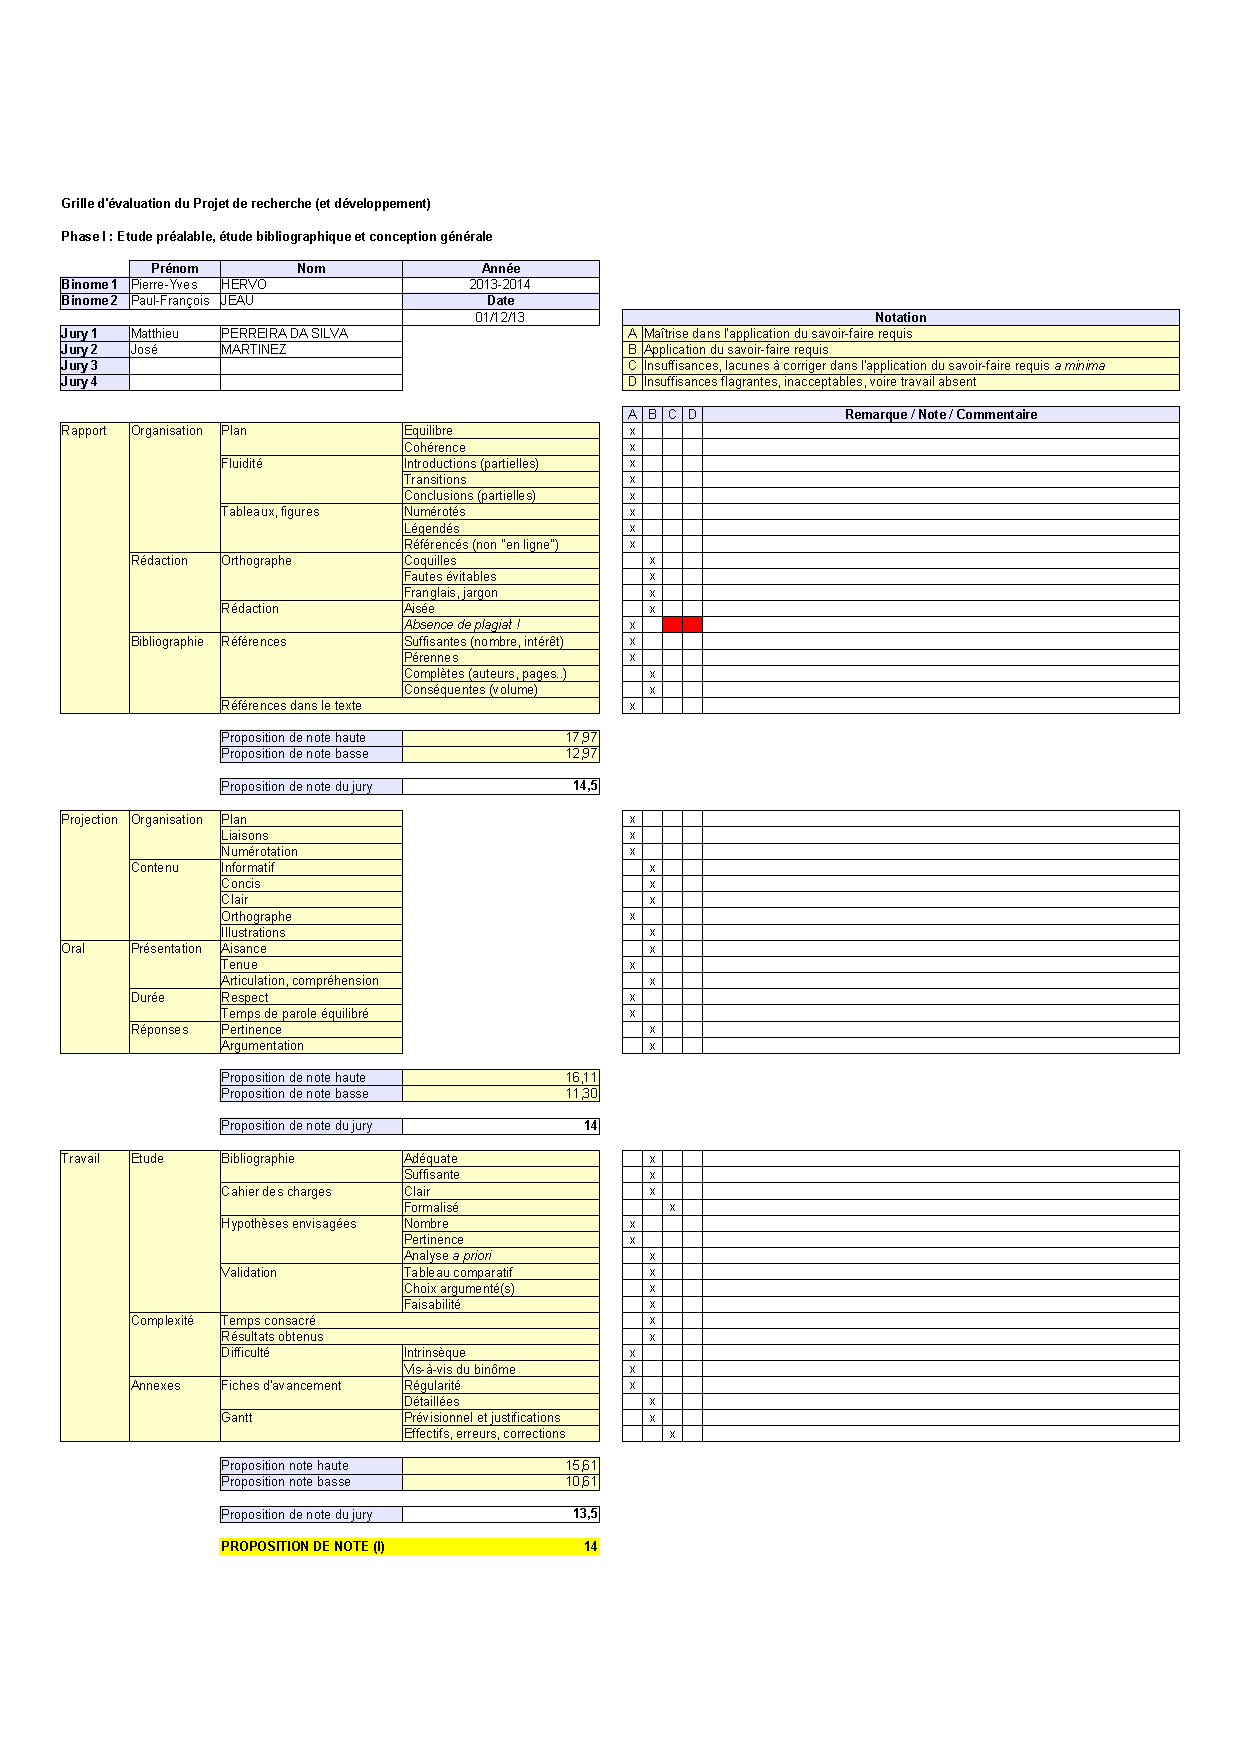
\includegraphics[width=0.9\textheight]{Images/Grille-Evaluation-PRD1}}
      \else
         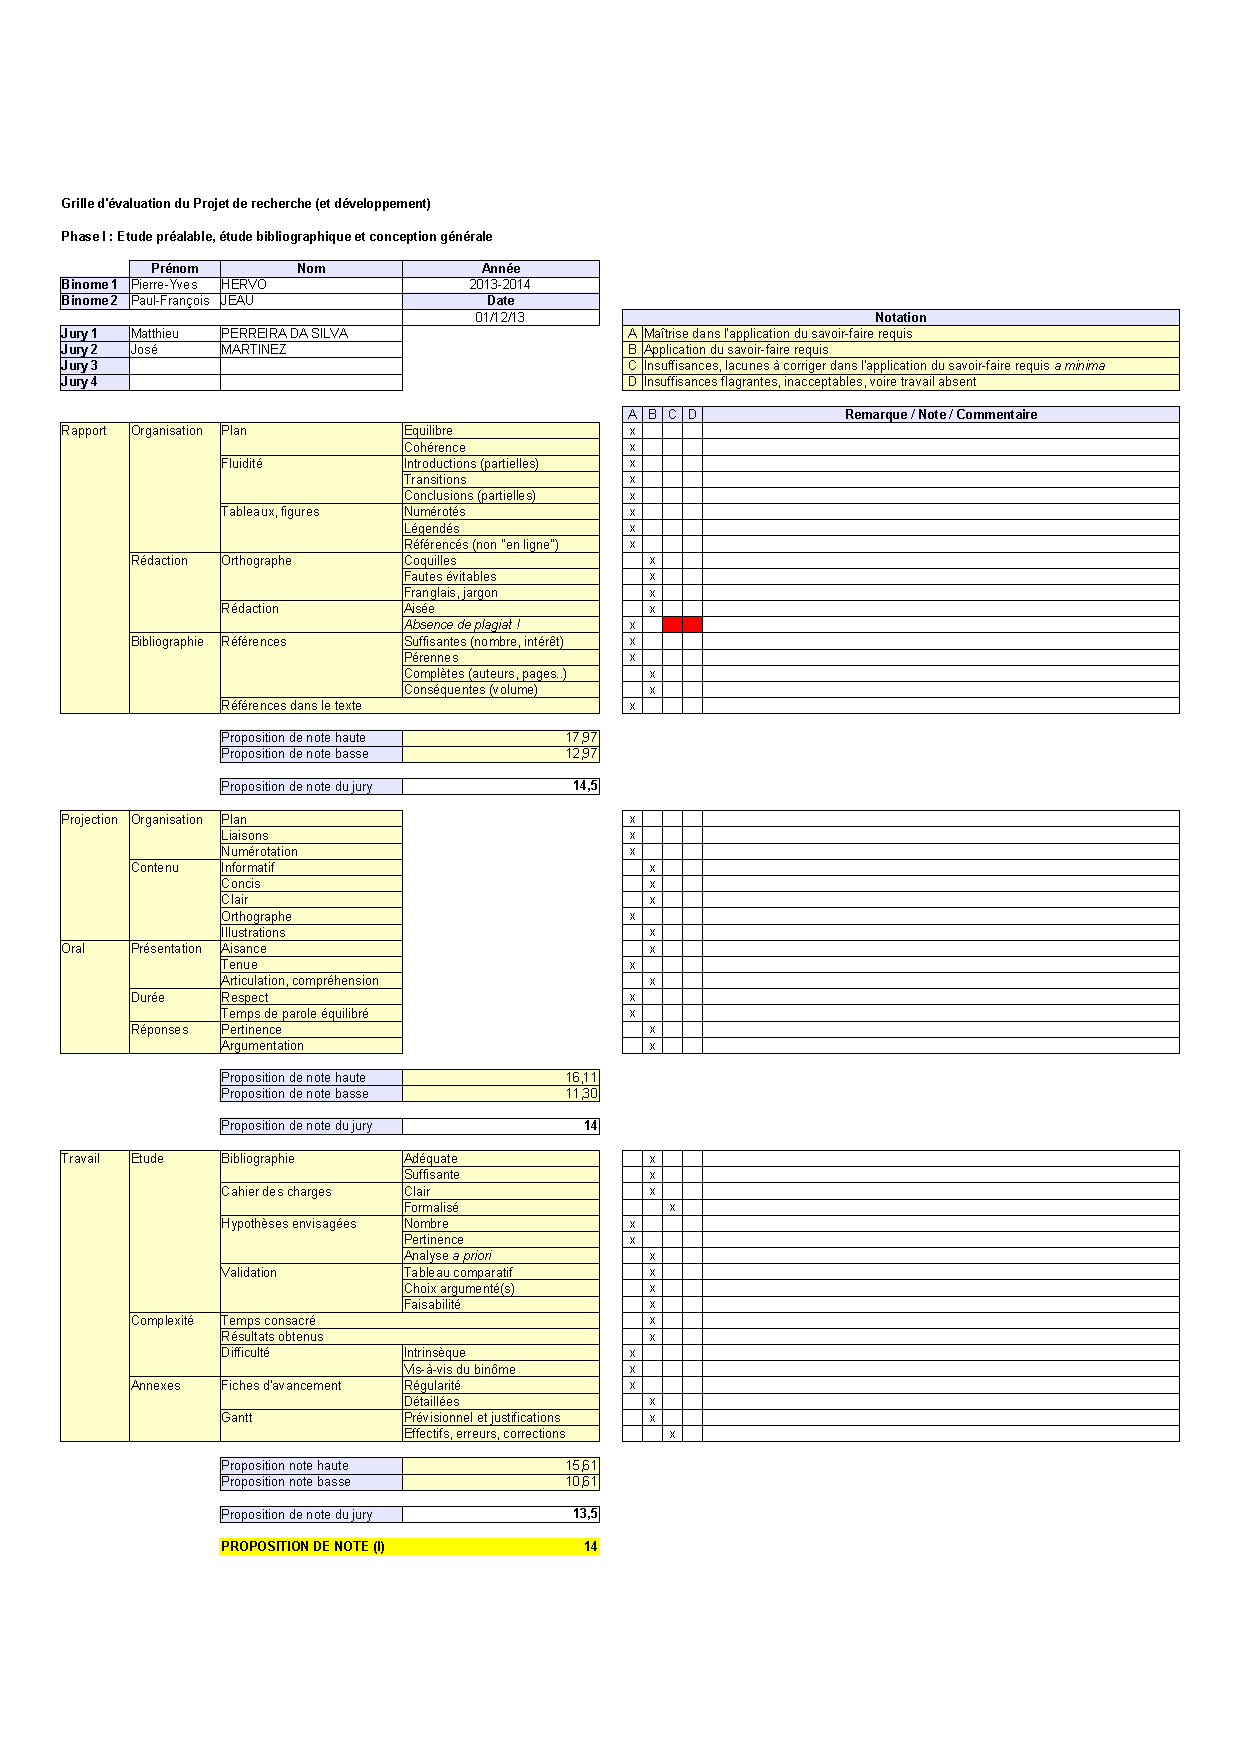
\includegraphics[width=0.9\textwidth]{Images/Grille-Evaluation-PRD1}
      \fi
	\caption{Points à contrôler à l'issue de la phase I}
	\label{fig:AutoEvaluationTravailIntermediaire}
\end{figure*}

La figure~\ref{fig:AutoEvaluationTravailFinal} permet d'énumérer un certain nombre de points importants dans les trois composantes du travail ainsi que d'évaluer notre niveau de satisfaction à l'issue de la phase~II, constituée de :
\begin{enumerate}
	\item la conception détaillée ;
	\item la réalisation ;
	\item la recette.
\end{enumerate}

\begin{figure*}
	\centering
      \ifscreen
         \rotatebox{90}{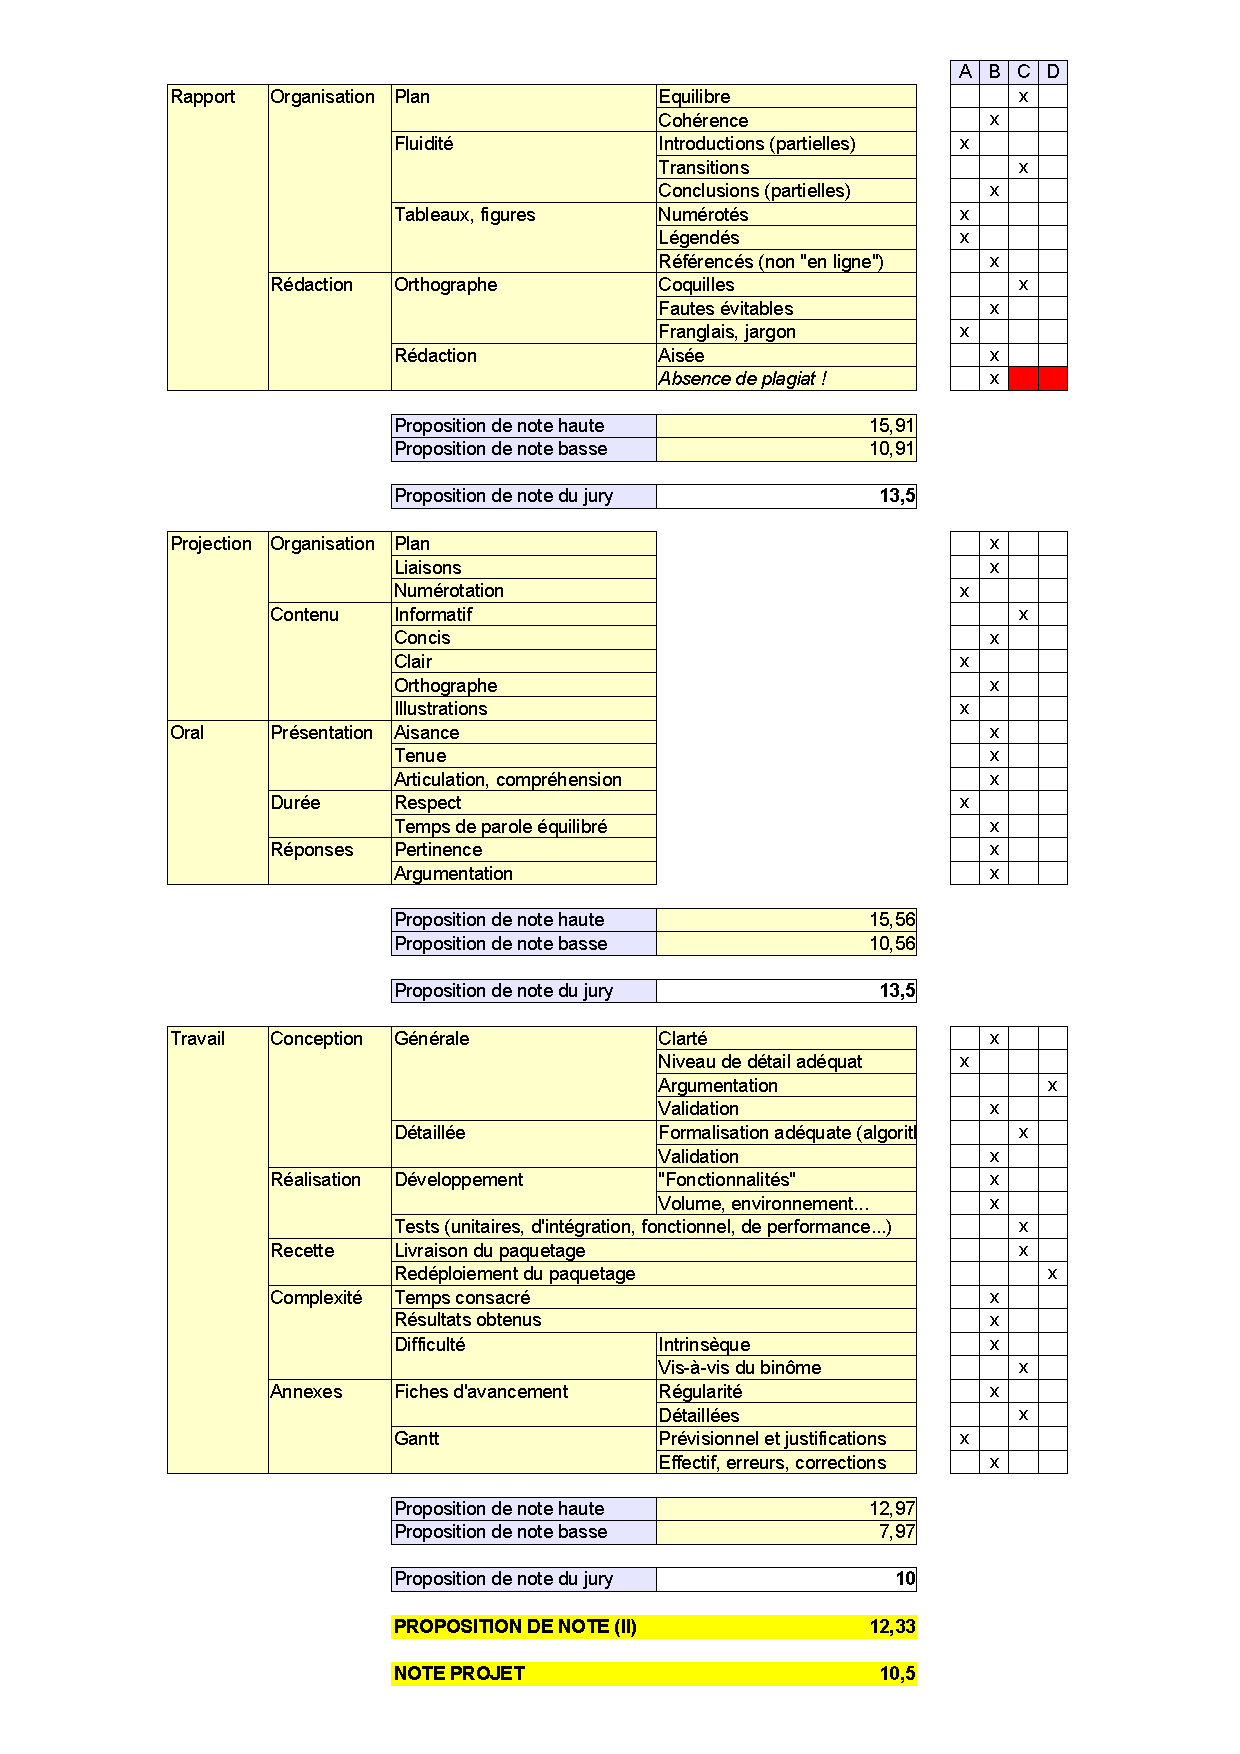
\includegraphics[width=0.9\textheight]{Images/Grille-Evaluation-PRD2}}
      \else
         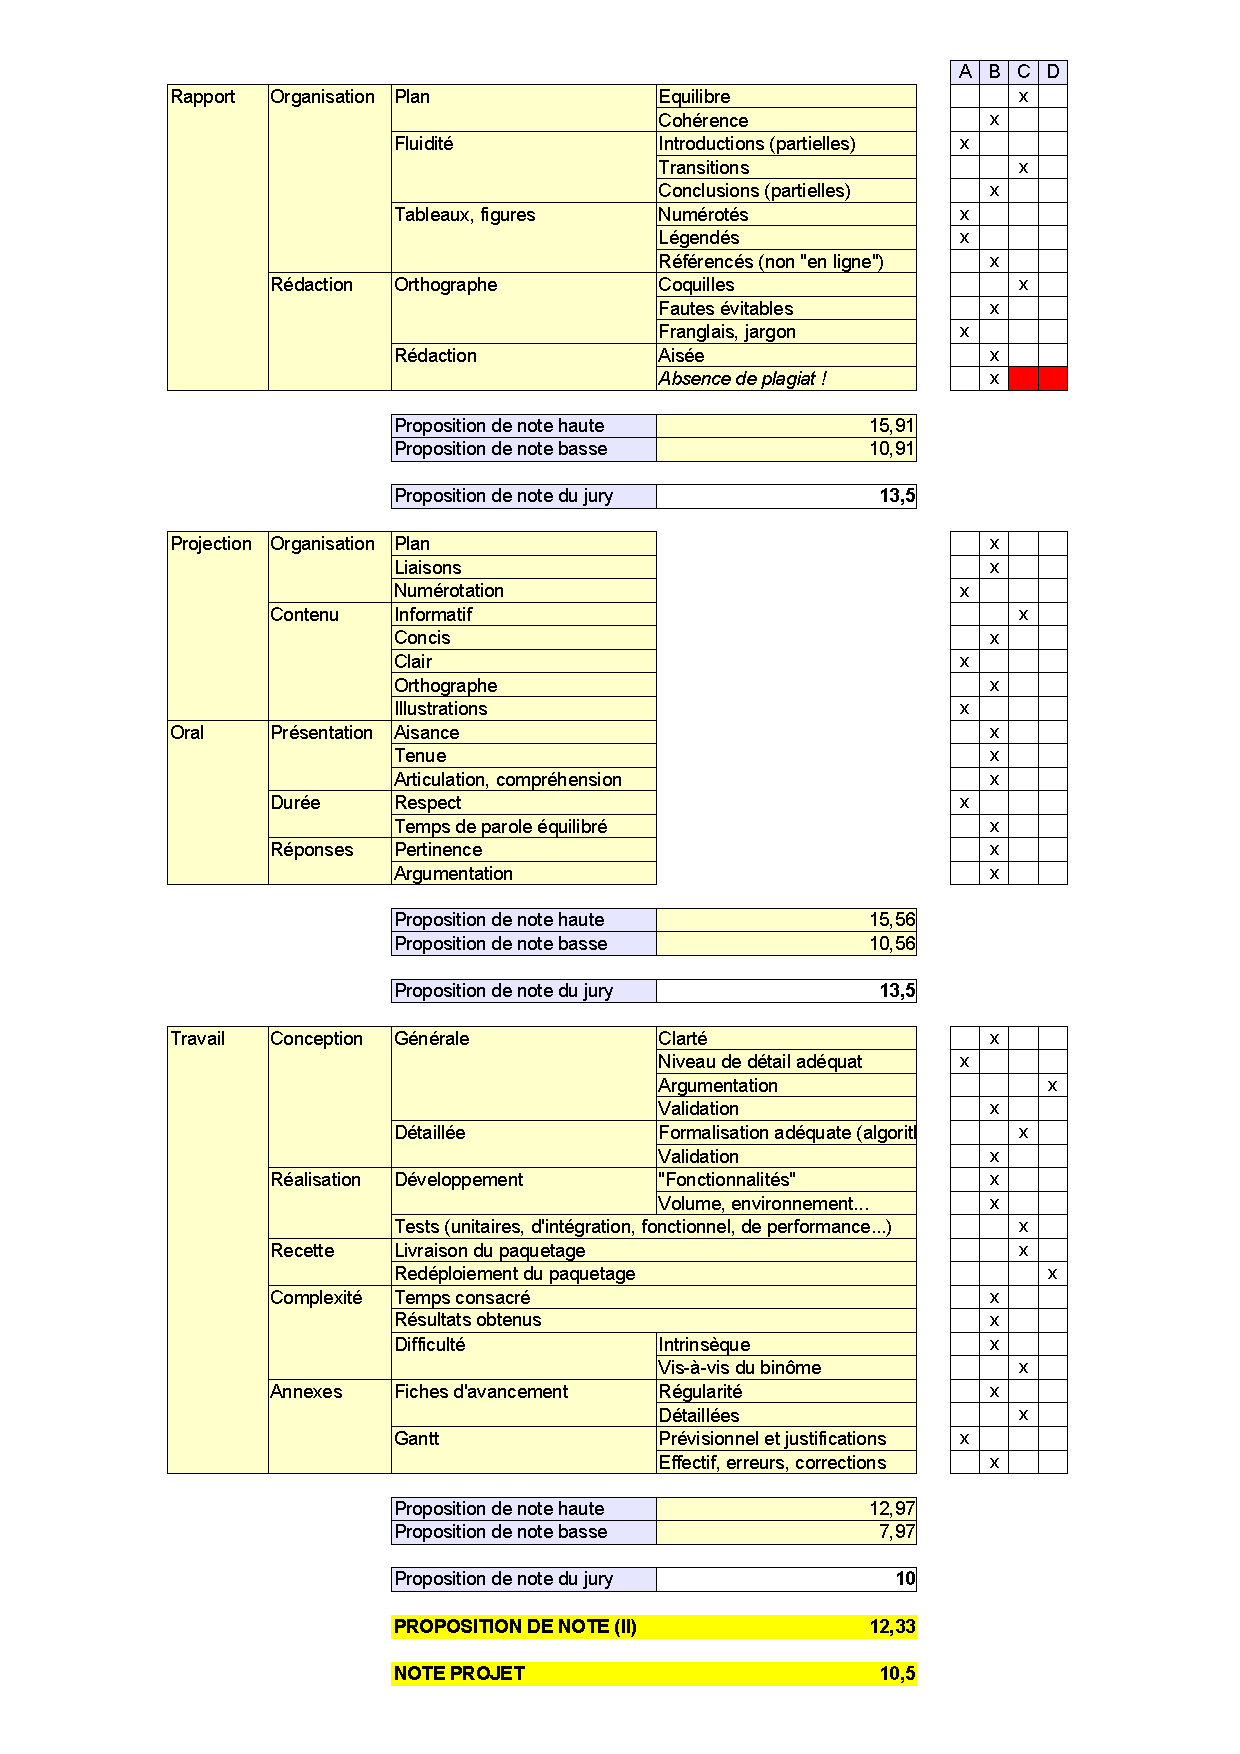
\includegraphics[width=0.9\textwidth]{Images/Grille-Evaluation-PRD2}
      \fi
	\caption{Points à contrôler à l'issue de la phase II}
	\label{fig:AutoEvaluationTravailFinal}
\end{figure*}

\end{document}
